% ------------------------------------------------------------------------
%
% -------------------      Plantilla_UIS.tex       -----------------------
%
% ------------------------------------------------------------------------
% ------------------------------------------------------------------------
% ------------------------------------------------------------------------
% Versión de plantilla para realización de informes de trabajo de grado
% construida para uso de la Universidad Industrial de Santander.
%
% Reservados todos los derechos
%
% Bucaramanga, Colombia
%
% Septiembre 17 de 2018
%
% ------------------------------------------------------------------------
% ------------------------------------------------------------------------
% ------------------------------------------------------------------------
%
% ------------------------------------------------------------------------
\documentclass[letter,oneside,12pt,spanish]{report}          % Encabezados
\usepackage[utf8]{inputenc}
%\usepackage[latin]{babel}
% ------------------------------------------------------------------------
\usepackage{icontec_style}                   % Libreria UIS ICONTEC
% ------------------------------------------------------------------------
% Ingrese en este punto las librerías específicas de usuario
% ------------------------------------------------------------------------
\usepackage{amsmath}
\usepackage{amssymb}
\usepackage{subfigure}
\usepackage{hyperref}
\usepackage{float}
\usepackage{graphicx}
\usepackage{algorithm,algpseudocode}
\usepackage{xcolor}
\setcounter{tocdepth}{4} % show also subsections in toc
\setcounter{secnumdepth}{4} % show also subsections number in toc
% ------------------------------------------------------------------------
% Archivo de bibliografía
% ------------------------------------------------------------------------
\addbibresource{references.bib}
% ------------------------------------------------------------------------
\def\autor{David Santiago Morales Norato}
\def\titulo{Algoritmo de clasificación de objetos en imágenes difractivas basado en medidas cuadráticas codificadas usando un enfoque de aprendizaje profundo}
\def\director{Andrés Felipe Jerez Ariza}
\def\codirector{Henry Arguello Fuentes}
\def\universidad{Universidad Industrial de Santander}
\def\escuela{Escuela de Ingeniería de Sistemas e Informática}
\def\facultad{Facultad de Ingenierías Fisicomecánicas}
\def\grupo{Grupo de Investigación en Diseño de Algoritmos y Procesamiento de Datos Multidimensionales (HDSP)}
\def\fecha{2022}
\def\codigo{2170102}

\DeclareMathOperator*{\minimize}{minimizar} % Declaración operador minimize

\DeclareMathOperator*{\maximize}{maximizar} % Declaración operador maximize
\DeclareMathOperator*{\subjectto}{sujeto \ a} % Declaración operador subjectto
\DeclareMathOperator*{\argmax}{arg \ max} % Declaración operador arg max

\DeclareMathOperator*{\argmin}{arg \ min} % Declaración operador arg min

\DeclareMathOperator*{\min}{min} % Declaración operador arg min

\newtheorem{definition}{Definición}% Declaración segmento definición matemática


% Traducción de palabras reservadas del algoritmo a español
\newenvironment{algoritmo}[1][]
  {\begin{algorithm}[#1]
     \selectlanguage{spanish}%
     \floatname{algorithm}{Algoritmo}%
     \renewcommand{\algorithmicif}{\textbf{si}}%
     \renewcommand{\algorithmicthen}{\textbf{entonces}}%
     \renewcommand{\algorithmicend}{\textbf{fin}}%
     \renewcommand{\algorithmicfor}{\textbf{para}}%
     \renewcommand{\algorithmicdo}{\textbf{hacer}}%
     % Set other language requirements
  }
  {\end{algorithm}}

\begin{document}       

% Inicio de documento
% ------------------------------------------------------------------------
% Definición silábica de palabras
% ------------------------------------------------------------------------
\hyphenation{pro-por-cio-nal di-se-ño}
\hypersetup {pdfborder = {0 0 0}}
% ------------------------------------------------------------------------
% Elementos previos al contenido del trabajo
% ------------------------------------------------------------------------
% ------------------------------------------------------------------------
%                                 Portada
% ------------------------------------------------------------------------

\thispagestyle{empty}

\begin{center}

\MakeUppercase{\titulo} \vspace{7cm}

\MakeUppercase{\autor}\\
\vspace{7cm}

\MakeUppercase{\universidad}\\
\MakeUppercase{\facultad}\\
\MakeUppercase{\escuela}\\
BUCARAMANGA\\
\fecha\\

\end{center}

% ------------------------------------------------------------------------
%                              Contraportada
% ------------------------------------------------------------------------

\newpage
\thispagestyle{empty}

\begin{center}

\MakeUppercase{\titulo} \vspace{2.3cm}

\MakeUppercase{\autor}\\
\vspace{2.3cm}

Trabajo de Grado para optar al título de\\
Ingeniero de Sistemas\\\vspace{1.5cm}

Director:\\
\director\\
Magíster en Matemática Aplicada\vspace{0.5cm}

Codirector:\\
\codirector\\
\textit{Ph.D. Electrical and Computer Engineering} \vspace{1.5cm}

\MakeUppercase{\universidad}\\
\MakeUppercase{\facultad}\\
\MakeUppercase{\escuela}\\
BUCARAMANGA\\
\fecha\\

\end{center}

% ------------------------------------------------------------------------
   % Portada, contraportada, formato de nota y autorización
% ------------------------------------------------------------------------
% ------------------------------------------------------------------------
% ------------------------------------------------------------------------
% ------------------------------------------------------------------------
%                               Dedicatoria
% ------------------------------------------------------------------------
% ------------------------------------------------------------------------
% ------------------------------------------------------------------------
\chapter*{DEDICATORIA}

 \begin{flushright}.
 
\textit{
Para mi mamá Mariana, mi papá Hanssel,\\ 
mis hermanas  María Silvana, Katherin y mi hermano Enrrique.\\
ellos son el círculo de personas que más amo.\\
Este trabajo de grado es el resultado de todo el esfuerzo y apoyo que mi familia me ha brindado, todo lo que soy y lo que seré, se lo debo a ellos.}
\end{flushright}


% ------------------------------------------------------------------------                                      % Dedicatoria
% ------------------------------------------------------------------------
% ------------------------------------------------------------------------
% ------------------------------------------------------------------------
% ------------------------------------------------------------------------
%                             AGRADECIMIENTOS
% ------------------------------------------------------------------------
% ------------------------------------------------------------------------
% ------------------------------------------------------------------------
\chapter*{AGRADECIMIENTOS}

Agradezco a mi director Andrés Jerez, una gran persona que me ha acompañado en mi formación tanto en lo académico como en lo personal, en especial le agradezco por su dedicación y paciencia como director de tesis.

Al grupo de investigación HDSP, por ser una comunidad de excelentes personas, las cuales me han brindado un gran apoyo tanto en lo académico como en lo personal desde mi vinculación al grupo.

A a la Universidad Industrial de Santander por ser la institución que me brindó lo necesario para crecer y formalizar mi curiosidad científica.

A Santiago y Ángela, su compañía, consejo y amistad ha marcado estos años.


% ------------------------------------------------------------------------
\newpage                              % Agradecimientos
% ------------------------------------------------------------------------
\tableofcontents                                      % Tabla de contenido
% ------------------------------------------------------------------------
\listoffigures                         % Lista de figuras, tablas y anexos
\listoftables
\listofanexo
% ------------------------------------------------------------------------
% ------------------------------------------------------------------------
% ------------------------------------------------------------------------
% ------------------------------------------------------------------------
%                                Glosario
% ------------------------------------------------------------------------
% ------------------------------------------------------------------------
% ------------------------------------------------------------------------
\chapter*{GLOSARIO}

% \begin{description}
%   \item[CONTROLADOR] (o también compensador) es un dispositivo que toma una decisión con base en la comparación de la información
%   medida con respecto a condiciones deseadas de operación. A dicha decisión se le denomina acción de control.
%   \item[CONTROLAR] es asignar valores a la variable manipulada para lograr que la variable controlada siga un valor de referencia.
%   \item[PERTURBACIÓN] señal indeseada que afecta negativamente el valor de la variable controlada del sistema.
%   \item[PID] sigla que refiere la acción combinada de control proporcional, integral y derivativo.
%   \item[SISTEMA] conjunto de elementos que interactúan de manera organizada para cumplir con un fin u objetivo común.
%   \item[VARIABLE CONTROLADA] es la cantidad o condición que se mide y controla.
%   \item[VARIABLE MANIPULADA] es la cantidad que el controlador modifica para afectar los valores de salida de la planta.
% \end{description}
% ------------------------------------------------------------------------                                % Glosario de términos
% ------------------------------------------------------------------------
% Contenido del Informe
% ------------------------------------------------------------------------
% ------------------------------------------------------------------------
% ------------------------------------------------------------------------
% ------------------------------------------------------------------------
%                                Resumen
% ------------------------------------------------------------------------
% ------------------------------------------------------------------------
% ------------------------------------------------------------------------
\chapter*{RESUMEN}

\footnotesize{
\begin{description}
  \item[TÍTULO:] \MakeUppercase{\titulo}
  \astfootnote{Trabajo de grado}
  \item[AUTOR:]\MakeUppercase{\autor} \asttfootnote{\facultad. \escuela. Director: \director. Codirector: \codirector}
  \item[PALABRAS CLAVE:] Palabras clave.
  \item[DESCRIPCIÓN:]\hfill \\ Resumen
\end{description}}\normalsize
% ------------------------------------------------------------------------                                                % Resumen

\chapter*{ABSTRACT}

\footnotesize{
\begin{description}
  \item[TITLE:] title\astfootnote{Bachelor Thesis}
  \item[AUTHOR:] \MakeUppercase{\autor} \asttfootnote{\facultad. \escuela. Advisor: \director. Co-advisor: \codirector}
  \item[KEYWORDS:] Key words.
  \item[DESCRIPTION:]\hfill \\ Abstract
\end{description}}\normalsize
% ------------------------------------------------------------------------                                               % Abstract
% ------------------------------------------------------------------------
% Capítulos
% ------------------------------------------------------------------------
% Introducción


\nnchapter{INTRODUCCIÓN}

Los algoritmos computacionales basados en aprendizaje profundo han sido ampliamente estudiados en la literatura, especialmente, la clasificación de objetos en imágenes ha sido una de las tareas computacionales más abordadas en ese tópico \myfootcite{li2019deep,li2018deep, wang2019development}. Los enfoques de aprendizaje profundo utilizan arquitecturas de redes neuronales, que consisten en la concatenación de múltiples capas compuestas de unidades mínimas llamadas neuronas. Cada neurona realiza una combinación lineal entre las entradas, para posteriormente usar una función no lineal en la salida. Las salidas de cada neurona en una capa funcionan como entrada de las neuronas ubicadas en la siguiente capa, creando así, una arquitectura de red neuronal profunda \myfootcite{fan2019selective}. 

En general, la clasificación de objetos se realiza sobre imágenes en escala de grises \myfootcite{bui2016using}, RGB \myfootcite{krizhevsky2017imagenet}, o más recientemente, imágenes espectrales \myfootcite{li2019deep}. Sin embargo, los enfoques de clasificación de objetos basados en aprendizaje profundo incorporan como entrada de la arquitectura de red neuronal, la información de la intensidad de la luz incidente sobre el sensor, omitiendo la información de fase, que resulta fundamental en aplicaciones como cristalografía de rayos-x \myfootcite{pinilla2018coded}, astronomía \myfootcite{fienup1987phase}, holografía \myfootcite{rivenson2018phase}, entre otras. Esta limitación se atañe a los sistemas ópticos que dependen de la conversión de fotones a electrones, puesto que no permiten una adquisición directa de la información de fase \myfootcite{shechtman2015phase}. Por lo tanto, la obtención de esta información de fase requiere la implementación de algoritmos computacionales que logren recuperar los datos perdidos.

Los algoritmos de recuperación de fase permiten reconstruir la información de un campo óptico inicial con base en la adquisición de medidas de intensidad que siguen un modelo cuadrático de propagación según diferentes campos de difracción, tales como campo cercano, medio y lejano \myfootcite{goodman2005introduction}. Dentro de estos sistemas ópticos de difracción se han incorporado máscaras de fase para la modulación del campo óptico inicial, puesto que, la literatura ha demostrado que la inclusión de este tipo de elementos ópticos durante el proceso de adquisición, genera redundancia en las medidas captadas, garantizando la recuperación de fase en hasta una constante unimodular \myfootcite{candes_CDP}. Estas medidas adquiridas a través de sistemas ópticos de difracción que incluyen máscaras de fase, se denominan medidas cuadráticas codificadas. Las imágenes recuperadas usando medidas cuadráticas codificadas se conocen como imágenes ópticas difractivas. Diversos algoritmos iterativos han sido propuestos para resolver la reconstrucción de imágenes difractivas a partir del problema de recuperación de fase. Tradicionalmente, estos algoritmos se construyen bajo formulaciones convexas, tales como el \textit{PhaseLift} \myfootcite{candes2013phaselift} y \textit{PhaseMax} \myfootcite{goldstein2018phasemax}; o formulaciones no convexas, tales como, \textit{Wirtinger Flow} \myfootcite{candes2015phase}, \textit{Truncated Wirtinger Flow} \myfootcite{chen2017solving}, \textit{Truncated Amplitude Flow} \myfootcite{wang2017solving} y \textit{Reweighted Amplitude Flow} \myfootcite{wang2018phase}.  

%\newpage
Actualmente, se han involucrado arquitecturas de redes neuronales profundas en el campo de formación de imágenes ópticas, puesto que, permite incorporar el modelo de adquisición como una capa de la misma arquitectura de red neuronal para promover una mejor reconstrucción de las medidas adquiridas. La inclusión del modelo de adquisición ha permitido el diseño de sistemas ópticos de adquisición a través de su implementación en configuraciones de red neuronal donde los pesos entrenables representan las variables optimizables del modelo de propagación \myfootcite{bacca2021transmittance}. 

Por otra parte, algunos trabajos han estudiado la clasificación de objeto usando únicamente medidas de intensidad captadas mediante sistemas ópticos definidos matemáticamente a través de operadores lineales, por ejemplo, sistemas de tomografía computarizada \myfootcite{douarre2020value}, imágenes de un solo píxel \myfootcite{bacca2020coupled}, entre otros. De manera que, los sistemas de clasificación que omiten el proceso de reconstrucción de las medidas obtenidas disminuyen el tiempo de inferencia, puesto que, se elimina la etapa de reconstrucción de la imagen, que generalmente, implica un alto costo computacional en los sistemas de clasificación. A pesar de que, se han desarrollado arquitecturas de redes neuronales para la clasificación usando medidas de intensidad bajo un modelo cuadrático \myfootcite{kim2018deep, ziletti2018insightful}, en la literatura de imágenes difractivas que resultan del problema de recuperación de fase no se han abordado modelos de redes neuronales para la detección de objetos basados en medidas cuadráticas codificadas. Así que, surge el interés de estudiar sistemas de clasificación que permitan la discriminación de objetos con base en medidas cuadráticas codificadas.

Por lo tanto, este trabajo de investigación propone el diseño de un algoritmo de clasificación de objetos en imágenes difractivas sobre medidas cuadráticas codificadas mediante el uso de aprendizaje profundo. La arquitectura de red neuronal de clasificación propuesta incluirá el modelo matemático que describe la adquisición de medidas cuadráticas para la clasificación de objetos en imágenes difractivas. Además, la evaluación de la arquitectura de red neuronal propuesta se realizará a través de bases de datos de la literatura y medidas simuladas. Asimismo, el algoritmo computacional de clasificación propuesto se comparará con técnicas del estado del arte.


Este documento se encuentra organizado de la siguiente manera: En sección 2, se describe el planteamiento del problema, incluyendo la justificación de este trabajo de investigación. La sección 3 presenta los objetivos tanto general como específicos de este trabajo. La sección 4 corresponde a la descripción de los conceptos generales y teóricos en relación con los sistemas ópticos de difracción, los algoritmos de recuperación de fase y sistemas de clasificación. La sección 5 describe la metodología planteada para alcanzar los objetivos propuestos. La sección 6 ilustra el cronograma de actividades que se realizarán durante el desarrollo del proyecto. Finalmente, la sección 7 describe el presupuesto del proyecto. 


%\pagebreak % Introducción
% ------------------------------------------------------------------------
% ------------------------------------------------------------------------
% ------------------------------------------------------------------------
%                              Objetivos
% ------------------------------------------------------------------------
% ------------------------------------------------------------------------
% ------------------------------------------------------------------------

\chapter{OBJETIVOS}

\subsection*{Objetivo general}

\begin{itemize}
   \item Desarrollar un algoritmo de clasificación de objetos en imágenes difractivas basado en medidas cuadráticas codificadas usando un enfoque de aprendizaje profundo.
\end{itemize}

\subsection*{Objetivos específicos}


\begin{itemize}

    \item Modelar matemáticamente el proceso de adquisición de medidas cuadráticas codificadas utilizando máscaras de fase.

    \item Diseñar e implementar un algoritmo de clasificación de objetos en medidas cuadráticas codificadas a partir de aprendizaje profundo que incorpore el modelo de adquisición.
    
    \item Simular una configuración óptica difractiva para la adquisición de medidas cuadráticas codificadas usando máscaras de fase.
    
    \item Evaluar el algoritmo de clasificación de medidas cuadráticas codificadas basado en aprendizaje profundo frente a otras técnicas del estado del arte usando medidas adquiridas con la configuración óptica simulada.

\end{itemize}
\pagebreak


% ------------------------------------------------------------------------
% ------------------------------------------------------------------------  % Objetivos
\chapter{ADQUISICIÓN DE LA INFORMACIÓN DE FASE}

Los sistemas ópticos tradicionales de adquisición captan únicamente la información de la intensidad de la luz incidente sobre el sensor, perdiendo la información de fase que resulta fundamental en aplicaciones, tales como cristalografía de rayos-x \myfootcite{pinilla2018coded}, astronomía \myfootcite{fienup1987phase}, holografía \myfootcite{rivenson2018phase}, entre otras. Por lo tanto, la obtención de la información de fase requiere la implementación  de sistemas ópticos que logren codificar la fase del campo óptico, preservándola implícita en las medidas de intensidad adquiridas. 
    
\section{SISTEMA ÓPTICO DE DIFRACCIÓN}
En múltiples áreas de la ciencia e ingeniería se presenta la adquisición de medidas cuadráticas de intensidad, con base en sistemas ópticos de difracción \myfootcite{fienup1987phase}$^,$\myfootcite{pinilla2018coded}$^,$\myfootcite{rivenson2018phase}. La Figura \ref{fig:difraction_systems} muestra un esquema convencional de los sistemas ópticos de difracción a lo largo de diferentes campos de propagación. Específicamente, este sistema de adquisición está compuesto por un objeto $\mathbf{z}\in\mathbb{C}^{n}$ ubicado en el campo óptico, que es iluminado por una fuente de luz coherente posteriormente, este campo óptico inicial se propaga una distancia $z$, produciendo medidas cuadráticas o patrones de difracción que, finalmente, se adquieren en el sensor. Cabe señalar que, se pueden definir tres diferentes campos de difracción $\psi$ según la distancia de propagación $z$, comúnmente conocidos como campo cercano, medio y lejano.

\begin{figure}[!h]
    \centering
    \caption{\hspace{2mm}Sistema óptico de difracción convencional.}
    \includegraphics[width=0.9\linewidth]{images/marco_teórico/diffraction_no_coded.pdf}
    \label{fig:difraction_systems}
\end{figure}

Matemáticamente, la adquisición de medidas cuadráticas $\mathbf{y}_{\psi}\in\mathbb{R}^n$ en cada campo de difracción $\psi$ se puede modelar como 

\begin{equation}
    \mathbf{y}_{\psi}= \vert \mathbf{A}_\psi \mathbf{z} \vert^2,
    \label{eq:diffraction_base}
\end{equation}

donde $\vert \cdot \vert$ denota la magnitud, y $\mathbf{A}_\psi\in\mathbb{C}^{n \times n}$ es la matriz que modela el sistema de adquisición según cada campo de difracción. Particularmente, el objeto de interés contiene información de magnitud y fase $\mathbf{z}=\vert \mathbf{z}|\odot e^{j\mathrm{ang}(\mathbf{z})}$ con $j=\sqrt{-1}$, donde $\mathrm{ang}(\cdot)$ devuelve la fase de un vector complejo. La matriz $\mathbf{A}_\psi$ se define como

\begin{equation}
    \mathbf{A}_\psi = \left\{\begin{matrix}
 \mathbf{F}\mathbf{T}\mathbf{F}^\mathcal{H}    & \text{si } \psi=1\rightarrow \text{Campo cercano}\\ 
 \mathbf{F}^\mathcal{H}\mathbf{Q} &\text{si } \psi=2\rightarrow\text{ Campo medio} \\ 
 \mathbf{F}  &\text{si } \psi=3\rightarrow\text{Campo lejano}
\end{matrix}\right., \label{eq:matrix_a_no_coded}
\end{equation}

donde $\mathbf{F}\in\mathbb{C}^{n\times n}$ corresponde a la transformada discreta de Fourier, $\mathbf{Q}\in\mathbb{C}^{n\times n}$ y $\mathbf{T}\in\mathbb{C}^{n\times n}$ representan matrices que describen las funciones de transferencia usadas en óptica de Fourier \myfootcite{poon2014introduction} para modelar la difracción en el campo cercano y medio, respectivamente, dadas por
\begin{equation}
(\mathbf{Q})_{p,q}=e^{\frac{-jk_0}{2z}(p^2\delta_x^2+q^2\delta_y^2)},\label{eq:Qfuncion}
\end{equation}
\begin{equation}
(\mathbf{T})_{r,s}=e^{-jk_0z\sqrt{1-\frac{(r\delta_{kx})^2}{k_0^2}-\frac{(s\delta_{ky})^2}{k_0^2}}}.\label{eq:Tfuncion}
\end{equation}
Aquí, $k_0=2\pi/\lambda$ representa el número de onda, $[p,q]$ y $[r,s]$ son los índices discretos de las muestras en el dominio espacial y el dominio de Fourier, respectivamente. Los términos $\delta_x$ y $\delta_y$ son el periodo de muestreo en las coordenadas espaciales, y $\delta_{kx}$ y $\delta_{ky}$ son el periodo de muestreo en las coordenadas de las frecuencias. 

% Es importante resaltar que en este documento, la notación de variables $x, y$ y $z$ hace referencia a coordenadas cartesianas, mientras que $\mathbf{x}, \mathbf{y}$ y $\mathbf{z}$ en negrita se refieren al objeto, las medidas cuadráticas, y la estimación del objeto, respectivamente.


\section{PROBLEMA DE RECUPERACIÓN DE FASE}

La recuperación del campo óptico inicial $\mathbf{z}$ usando medidas cuadráticas es un problema inverso comúnmente denominado recuperación de fase. En general, el problema de recuperación de fase basado en \eqref{eq:diffraction_base} se puede definir como 

\begin{equation}
    \minimize_{\mathbf{z}\in\mathbb{C}^n}\Vert\mathbf{y}_{\psi} - \vert \mathbf{A}_{\psi}\mathbf{z} \vert\Vert_2^2, 
    \label{eq:phase_retrieval_problem}
\end{equation}

donde $\Vert \cdot\Vert_2$ es la norma euclidiana. Usualmente, se puede garantizar una recuperación que conserva un error de fase global \eqref{eq:phase_retrieval_problem} \myfootcite{eldar2014phase}$^,$\myfootcite{ gross2017improved}$^,$\myfootcite{ 9062527}, es decir que, $\hat{\mathbf{z}} = \hat{\mathbf{z}}e^{j\theta}$ con $\theta \in [0, 2\pi)$. En consecuencia, la distancia euclidiana entre la escena $\mathbf{z}$ y su estimación $\hat{\mathbf{z}}$ está dada por
\begin{equation}
    \mathrm{dist}(\mathbf{z}, \hat{\mathbf{z}}) = \min_{\theta \in [0, 2\pi)}\Vert \mathbf{z}e^{-j\theta} - \tilde{\mathbf{z}}\Vert_2.
\end{equation}

Adicionalmente, el problema inverso \eqref{eq:phase_retrieval_problem} se ha resuelto creando redundancia en el proceso de medición al incluir una máscara de fase, que permite la modulación del campo óptico, produciendo medidas cuadráticas codificadas según cada campo de difracción.

% Cabe señalar que, la información de fase en el plano Fourier es de suma importancia para garantizar la recuperación de la señal adquirida. La Figura \ref{fig:mescla_fases} ilustra un experimento desarrollado en \myfootcite{shechtman2015phase} donde se intercambia la información de fase de la transformada de Fourier de dos imágenes, posteriormente, se aplica la transformada de Fourier inversa a este intercambio. Aquí, se puede observar que en la imagen resultante predomina la información de las fases contrarias.

% \begin{figure}[!h]
%     \centering
%     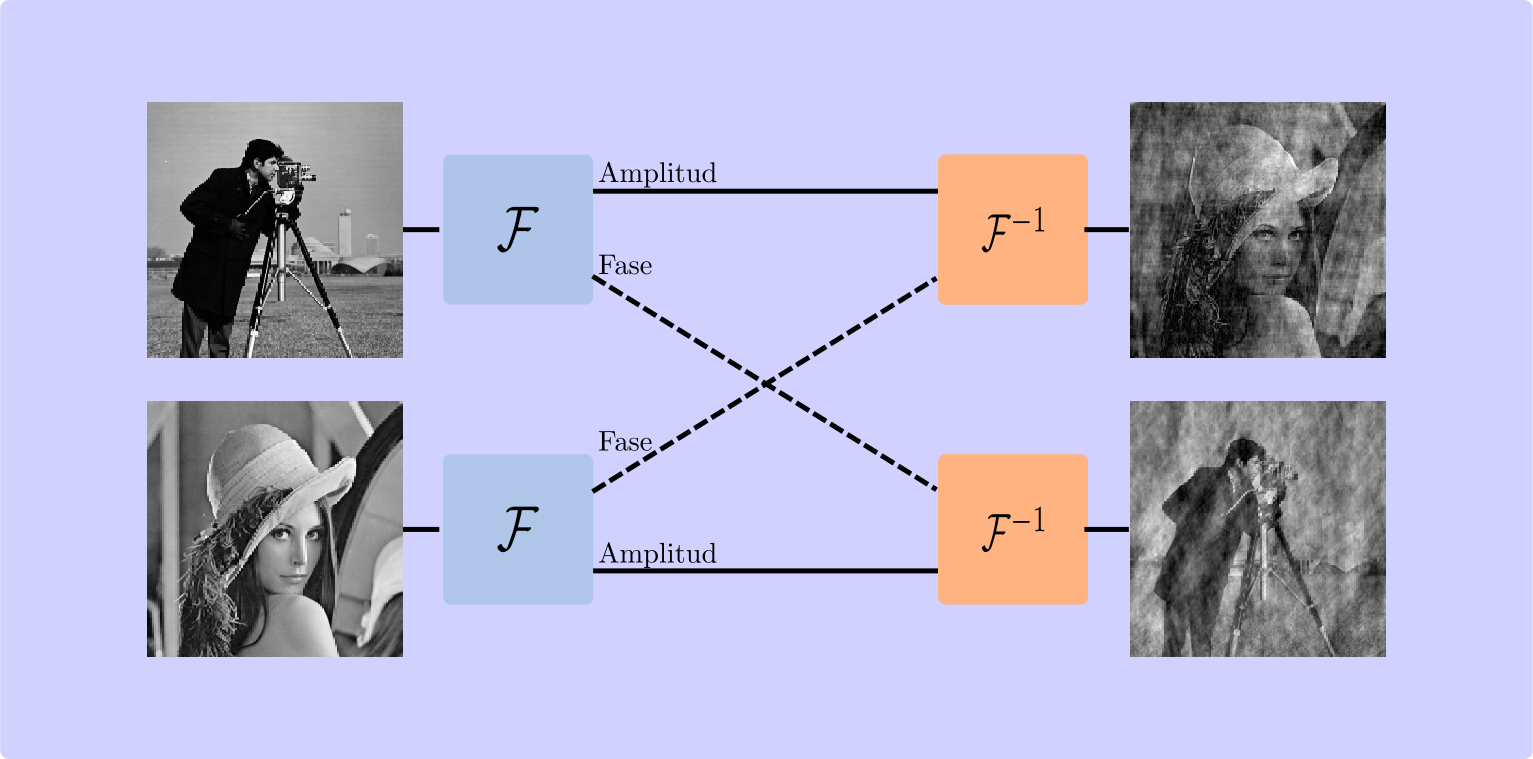
\includegraphics[width=0.9\linewidth]{images/marco_teórico/mescla_abs_fase.pdf}
%     \caption{\hspace{2mm}Experimento intercambiando la información de fase de la transformada de Fourier.}
%     \label{fig:mescla_fases}
% \end{figure}


% \pagebreak
\section{MEDIDAS CUADRÁTICAS CODIFICADAS}
En esta subsección, se describe el sistema de adquisición que capta medidas cuadráticas codificadas de un campo óptico a lo largo de cada campo de difracción. La Figura \ref{fig:coded_difraction_systems} ilustra el esquema de adquisición de medidas cuadráticas codificadas que incluye una máscara de codificación de fase $\mathbf{D}_\ell \in \mathbb{C}^{n\times n}$ para modular el campo óptico inicial. De hecho, al modificar la configuración espacial de la máscara de fase es posible adquirir múltiples proyecciones de la escena. De modo que, las proyecciones cuadráticas codificadas en cada campo de difracción para la $\ell$-ésima proyección está dada por 
\begin{equation}
    \mathbf{y}_{\ell, \psi} = \vert \mathbf{A}_{\ell, \psi}\mathbf{z} \vert, \ell=\{1,\dots,L\},
    \label{eq:phase_retrieval_problem}
\end{equation}

donde $\mathbf{A}_{\ell, \psi}\in\mathbb{C}^{n\times n}$ es la matriz que describe la $\ell$-ésima proyección según la propagación de cada campo de difracción $\psi$, siendo $L$ el número total de proyecciones. 
\begin{figure}[!h]
    \centering
    \caption{\hspace{2mm}Sistema óptico de difracción codificado.}
    \includegraphics[width=0.9\linewidth]{images/marco_teórico/diffraction_coded.pdf}
    \label{fig:coded_difraction_systems}
\end{figure}

Específicamente, la matriz del sistema de adquisición $\mathbf{A}_{\ell, \psi}$ introduciendo una máscara de fase, se puede expresar como

\begin{equation}
    \mathbf{A}_{\ell,\psi}= \left\{\begin{matrix}
\mathbf{F}\mathbf{T}\mathbf{F}^\mathcal{H} \mathbf{D}_\ell  & \text{si } \psi=1\rightarrow \text{Campo cercano}\\ 
\mathbf{F}^\mathcal{H}\mathbf{Q}\mathbf{D}_\ell &\text{si } \psi=2\rightarrow\text{ Campo medio} \\ 
\mathbf{F}\mathbf{D}_\ell  &\text{si } \psi=3\rightarrow\text{Campo lejano}
\end{matrix}\right.. \label{eq:matrix_a}
\end{equation}
En general, las entradas aleatorias de la matriz  $\mathbf{D}_{\ell} = \mathrm{diag}(\mathbf{d})$ son $i.i.d$ copias de una variable aleatoria $d \in \mathbb{C}$ con $\mathbf{d} \in \{d\}^{n}$, donde $\mathrm{diag}(\cdot)$ devuelve una matriz diagonal cuadrada de un vector dado. Aquí, $d$ representa una modulación pasiva en la fase, por lo tanto, se impone que $d$ no aumenta la energía de la escena durante el proceso de modulación. Así que, se establece la Definición \ref{def:admissible} para garantizar la admisibilidad de la variable aleatoria.

\begin{definition}{(Variable aleatoria admisible). \myfootcite{9062527}} 
    Una variable aleatoria que cumple con $|d|\leq 1$, se considera admisible como elemento de modulación en fase.\label{def:admissible}
\end{definition}


Algunos ejemplos de variables aleatorias que satisfacen la Definición \ref{def:admissible} se listan en la Tabla \ref{tab:admi_examples}. Estas variables aleatorias han sido usados en \myfootcite{9062527} como elementos de codificación para resolver el problema de recuperación de fase.

\begin{table}[!h]
\centering
\caption{Ejemplos de codificaciones aleatorias admisibles según la Definición \ref{def:admissible}.}
\begin{tabular}{|c|c|}
\hline
\textbf{Elemento de codificación} & \textbf{Probabilidad}                     \\ \hline
$d \in \{0, 1\}$         & $\{ \frac{1}{2},  \frac{1}{2}\}$ \\ \hline
$d \in \{-1, 1\}$        & $\{ \frac{1}{2},  \frac{1}{2}\}$ \\ \hline
$d \in \{-1, 1, -j,  j\}$ & $\{ \frac{1}{4},  \frac{1}{4}, \frac{1}{4},  \frac{1}{4}\}$ \\ \hline
\end{tabular}
\label{tab:admi_examples}
\end{table}

% Cabe destacar que, en este trabajo de investigación se emplearon máscaras aleatorias con valores de $d \in \{-1, 1, -j,  j\}$, debido a sus características estadísticas \myfootcite{9062527}.

% \begin{equation}
%     \vert d \vert \leq M, \quad \mathbb{E}[d] = 0, \quad  \mathbb{E}[d^2] = 0, \quad  \mathbb{E}[\vert d \vert^4] = 2\mathbb{E}[\vert d \vert^2]^2,    
%     \label{eq:restricciones_mascara}
% \end{equation}

% donde $\mathbb{E}[\cdot]$ corresponde al valor esperado. Aquí, se busca que $M=1$ para que la codificación no incremente la potencia de las medidas cuadráticas.

\chapter{ALGORITMOS DE RECUPERACIÓN DE FASE}
En esta sección, se presentan los algoritmos comúnmente utilizados para recuperar el campo óptico inicial a partir de medidas cuadráticas codificadas. La literatura ha planteado diferentes algoritmos basados en formulaciones convexas y no convexas como se expone a continuación.

\section{FORMULACIONES CONVEXAS}

Este tipo de algoritmos relajan el problema de recuperación de fase a un problema convexo equivalente.

\begin{itemize}
    \item \textbf{PhaseLift \myfootcite{candes2013phaselift}}:
    este algoritmo plantea el problema de recuperación de fase como una minimización de la traza de la siguiente forma
    \begin{equation}
        \begin{aligned}
            \minimize_{\mathbf{z} \in \mathbb{C}^{n}} \quad & \quad \mathrm{Traza}(\mathbf{z}\mathbf{z}^{\mathcal{H}}), \\
            \subjectto \quad & \quad \mathcal{A}(\mathbf{z}\mathbf{z}^{\mathcal{H}}) = \mathbf{b}, \\
             &\quad  \mathbf{z}\mathbf{z}^{\mathcal{H}} \succ 0,
        \end{aligned}
    \end{equation}
    
    donde $\mathcal{A}( \cdot ): \mathbb{R}^{n} \rightarrow \mathbb{R}^{m}$ es un operador lineal y $\mathrm{Traza}(\cdot)$ representa la traza de una matriz.
    
    \item \textbf{PhaseMax} \myfootcite{goldstein2018phasemax}:
    sea $\mathbf{\hat{z}} \in \mathbb{C}^{n}$ un vector aproximación de la señal original $\mathbf{z}$, de modo que, la señal reconstruida se obtiene solucionando el siguiente problema convexo
        
    \begin{equation}
        \begin{aligned}
            \maximize_{\mathbf{z}\in \mathbb{C}^n} \quad & \langle \mathbf{z}, \mathbf{\hat{z}} \rangle_{\mathbb{R}}, \\
            \subjectto \quad & \vert \langle \mathbf{a}_i,\mathbf{z} \rangle \vert \leq (\boldsymbol{\phi})_i,
        \end{aligned}
    \end{equation}
    donde $\langle \cdot, \cdot \rangle_{\mathbb{R}}$ denota la parte real del producto interno y $(\boldsymbol{\phi})_i = \sqrt{(\mathbf{y})_i}$.
    
\end{itemize}

\section{FORMULACIONES NO CONVEXAS}
Las formulaciones no convexas requieren una estimación inicial de la escena o inicialización, además, calculan el gradiente siguiendo la diferenciación de Wirtinger.
\begin{itemize}
    \item \textbf{TRUNCATED WIRTINGER FLOW (TWF) \myfootcite{chen2017solving}:} este algoritmo se basa en el modelo de muestreo según unas variables aleatorias que siguen una distribución de Poisson, de la forma
    
    \begin{equation}
        (\mathbf{y})_i\sim \mathrm{Poisson}( \vert \langle \mathbf{a}_i,\mathbf{z}\rangle \vert^2 ), \quad i=1,\dots,m.
    \end{equation}
    
    TWF busca minimizar la máxima estimación de probabilidad 
    
    \begin{equation}
        \minimize_{z \in \mathbb{C}^{n}} - \sum_{i=1}^{m} \ell(\mathbf{z};\mathbf{y}_i),
    \end{equation}
    
    donde $\ell(\mathbf{z};\mathbf{y}_i) = { \mathbf{y}_i\log(|\mathbf{a}_i^H \mathbf{z}|^2) -|\mathbf{a}_i^H \mathbf{z}|^2 }$ con $(\cdot)^H$ el operador de conjugada transpuesta
    
    \item \textbf{TRUNCATED AMPLITUDE FLOW (TAF) \myfootcite{wang2017solving}:} este algoritmo adopta un criterio de mínimos cuadrados para recuperar $\mathbf{z}$ basado en las medidas sin fase $\mathbf{y}$ 
    
    \begin{equation}
        \minimize_{\mathbf{z} \in \mathbb{C}^{n}} \frac{1}{2m} \sum_{i=1}^{m} (\vert \langle \mathbf{a}_i,\mathbf{z}\rangle \vert - (\boldsymbol{\phi})_i)^2,
    \end{equation}
    
    Este algoritmo asume que las medidas $\mathbf{y}_i$ provienen de un sistema gaussiano de la forma $\mathbf{y}_i \sim \mathcal{N}(\vert \langle \mathbf{a}_i,\mathbf{z}\rangle \vert^2, 1)$
    
    \item \textbf{REWEIGHTED AMPLITUDE FLOW (RAF) \myfootcite{wang2018phase}:} este algoritmo sigue el criterio de maximizar la estimación de probabilidad de la forma
    
    \begin{equation}
        \minimize_{z \in \mathbb{C}^{n}} -\sum_{i=1}^{m} \ell(\mathbf{z};(\boldsymbol{\phi})_i/(\mathbf{y})_i),
    \end{equation}
    
    donde en el caso de un muestreo con ruido gaussiano basado en la amplitud $\ell(\mathbf{z};\mathbf{y}_i) = (\vert \langle \mathbf{a}_i,\mathbf{z}\rangle \vert - (\boldsymbol{\phi})_i)^2$ o basado en la intensidad  $\ell(\mathbf{z};(\mathbf{y})_i) = (\vert \langle \mathbf{a}_i,\mathbf{z}\rangle \vert^2 - (\mathbf{y})_i)^2$. Por otra parte, basado en un muestreo con distribución de Poisson, $\ell(\mathbf{z};(\mathbf{y})_i) = {(\mathbf{y})_i \log(|\mathbf{a}_i^H \mathbf{z}|^2) -|\mathbf{a}_i^H \mathbf{z}|^2 }$ 
\end{itemize}





\chapter{SISTEMAS DE CLASIFICACIÓN}

La clasificación ha sido una de las tareas computacionales más abordadas en el estado del arte. Específicamente, dentro de los algoritmos de clasificación tradicionales se encuentran las máquinas de soporte vectorial, K vecinos más cercanos \myfootcite{kim12012comparing} y los enfoques basados en redes neuronales \myfootcite{li2019deep}$^,$\myfootcite{li2018deep}$^,$\myfootcite{ wang2019development}, los cuales se describen a continuación.
\section{MÁQUINAS DE SOPORTE VECTORIAL}
Las máquinas de soporte vectorial (SVM, de su sigla en inglés, \textit{support vector machine}) \myfootcite{suthaharan2016support} permiten la clasificación binaria, donde cada punto $n$-dimensional $\mathbf{x}_i$ tiene asociada una etiqueta de clase $c_i \in \{1,-1\}$.

Suponiendo que los datos de ambas clases son separables linealmente, este método propone separar los datos usando el hiperplano $\mathbf{w}\mathbf{x}_i + b = 0$. En la Figura \ref{fig:svm} se muestra una representación de una SVM en $\mathbb{R}^2$

\begin{equation}
    \begin{split}
        \mathbf{w}\mathbf{x}_i + b &\geq 1 \quad si \quad c_i=1, \\
        \mathbf{w}\mathbf{x}_i + b &\leq 1 \quad si \quad c_i=-1.
    \end{split}
\end{equation}

Cabe resaltar que, para todos los elementos del conjunto de datos se cumple que

\begin{equation}
    c_i(\mathbf{w}\mathbf{x}_i + b) \geq 1, \quad i=1,\dots, m.
\end{equation}

\begin{figure}[H]
    \centering
    \caption{\hspace{2mm}Representación de una SVM en $\mathbb{R}^2$. La recta $\mathbf{wx} -b = 0$ en rojo representa el plano óptimo que soluciona el problema de optimización \eqref{eq:problema_optimización_svm}. Las rectas $\mathbf{wx} -b = 1$ y $\mathbf{wx} -b = -1$ representan los extremos de separación de las clases de puntos en rojo y en azul.}
    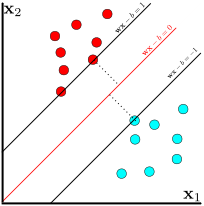
\includegraphics[width=0.4\linewidth]{images/marco_teórico/svm.pdf}
    \label{fig:svm}
\end{figure}

El problema de optimización se plantea de la siguiente forma

\begin{equation}
    \begin{aligned}
        \minimize_{\mathbf{w}} & \quad \Vert \mathbf{w} \Vert, \\
        \subjectto_{\quad i=1,\dots, m} & \quad c_i(\mathbf{w}\mathbf{x}_i + b) \geq 1.
    \end{aligned}
    \label{eq:problema_optimización_svm}
\end{equation}

Usualmente, no es posible separar los datos de forma lineal, por esta razón, se puede incluir una función no lineal $ \phi$ que transforme los datos a un conjunto de características donde las clases sean separables linealmente. El problema de optimización para una SVM usando un kernel $\phi$ se formula como

\begin{equation}
    \begin{aligned}
        \minimize_{\mathbf{w}} & \quad \Vert \mathbf{w} \Vert, \\
        \subjectto_{\quad i=1,\dots, m} & \quad c_i(\mathbf{w}\phi(\mathbf{x}_i) + b) \geq 1.
    \end{aligned}
\end{equation}


\section{K VECINOS MÁS CERCANOS}

K vecinos más cercanos (KNN, por sus siglas en inglés, \textit{k-nearest neighbors.}) propone que un conjunto $D = \{(\mathbf{x}_i, {c}_i)\}_1^n$, siendo $\mathbf{x}_i$ el vector de características y $\mathbf{c}_i$ la clase correspondiente. Para un nuevo vector a clasificar $\mathbf{\hat{x}}$, el algoritmo KNN encuentra los $K$ puntos más cercanos del conjunto de datos. La Figura \ref{fig:knn} muestra una representación de la clasificación de dos nuevas muestras en $\mathbb{R}^2$ con $K = 5$. Tradicionalmente, se emplea la distancia euclidiana 

\begin{equation}
    d(\mathbf{x}_p,\mathbf{x}_q) = \Vert \mathbf{x}_p-\mathbf{x}_q \Vert_2
    \label{eq:distancia_euclidiana}
\end{equation}

\begin{figure}[H]
    \centering
    \caption{\hspace{2mm}Representación de KNN en $\mathbb{R}^2$ con $K = 5$.}
    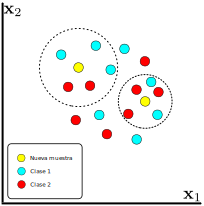
\includegraphics[width=0.4\linewidth]{images/marco_teórico/knn.pdf}
    \label{fig:knn}
\end{figure}

Posteriormente, con base en las clases de los $K$ puntos encontrados, de tal forma que, $C \subset D$ y $\vert C \vert = K$, se cuantifica la cantidad de veces que aparece cada clase y se clasifica la nueva muestra $\mathbf{\hat{x}}$ con la clase que más veces aparezca de la forma

\begin{equation}
    \mathrm{clase}(\mathbf{\hat{x}}) =  \argmax_{\hat{c}} \bigg\{ \sum_{\hat{c} \in C} \delta(C,\hat{c})\bigg\},
\end{equation}

donde $\delta(\cdot,\cdot)$ corresponde a la función delta de Kronecker, dada por

\begin{equation}
    \delta(a,b) = \begin{cases}
        1, \quad a = b \\
        0, \quad a \neq b
    \end{cases}
\end{equation}
\section{REDES NEURONALES}

Los enfoques de aprendizaje profundo han generado un gran progreso en el desarrollo de problemas muy complejos en los últimos años
\myfootcite{he2016deep}$^,$\myfootcite{li2019deep}$^,$\myfootcite{li2018deep}$^,$\myfootcite{wang2019development}$^,$\myfootcite{vaswani2017attention}. El aprendizaje profundo busca encontrar una función $f: \mathbb{R}^{d_1} \rightarrow \mathbb{R}^{d_2}$ que relacione un dato de entrada con una respectiva salida. La función $f$ comúnmente se denomina arquitectura de red neuronal profunda, puesto que, consiste en la concatenación de múltiples capas compuestas por unidades mínimas llamadas neuronas. Cada neurona realiza una combinación lineal entre las entradas, posteriormente, se emplea una función no lineal en la salida. Las salidas de cada neurona en una capa funcionan como entrada de las neuronas ubicadas en la siguiente capa, por lo tanto, se construye una arquitectura de red neuronal profunda \myfootcite{fan2019selective}. En la Figura \ref{fig:nn}, se muestra una arquitectura de red neuronal $f: \mathbb{R}^{d_1} \rightarrow \mathbb{R}^{d_2}$.

\begin{figure}[H]
    \centering
    \caption{\hspace{2mm}Esquema de una arquitectura de red neuronal $f: \mathbb{R}^{d_1} \rightarrow \mathbb{R}^{d_2}$.}
    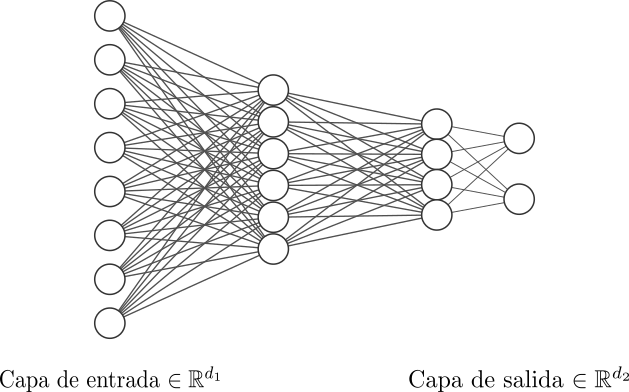
\includegraphics[width=0.6\linewidth]{images/marco_teórico/nn.pdf}
    \label{fig:nn}
\end{figure}

Por otra parte, el modelo matemático de una red neuronal estándar se puede definir como
\begin{equation}
    \footnotesize 
    \big\{f_\theta(\mathbf{x}) = \sigma_{J}(\mathbf{W}_{J}\sigma_{J-1}(\mathbf{W}_{J-1} (\dots \sigma_2(\mathbf{W}_2\sigma_1(\mathbf{W}_1\mathbf{x} + \mathbf{b}_1) + \mathbf{b}_2))  + \mathbf{b}_{J-1})  + \mathbf{b}_J) \quad \vert \quad\theta = \{\mathbf{W}_{j}, \mathbf{b}_{j}\}  \big\},
    \label{eq:red_neuronal}
\end{equation}

donde $1 \leq j \leq J$ representa cada una de las capas que compone la red neuronal, $\sigma_j$ corresponde a una función no lineal en dicha capa, $\mathbf{W}_j$ es la matriz de pesos y $\mathbf{b}_j$ es el bias de la capa. Con el fin de entrenar los pesos $\theta$ bajo un enfoque de aprendizaje supervisado, se requiere de un conjunto de entrenamiento $\{(\mathbf{x}_k, c_k) \}_{k=1}^{N}$ y una función de costo $\mathcal{L}( c_k,  f_\theta(\mathbf{x}_k))$ para plantear el problema de optimización 

\begin{equation}
    \minimize_\theta \frac{1}{N}\sum_{k=1}^{N} \mathcal{L}( {c}_k,  f_\theta(\mathbf{x}_k)).
    \label{eq:optimización_nn}
\end{equation}
\section{CLASIFICACIÓN DE IMÁGENES USANDO REDES NEURONALES ÓPTICAS}


Recientemente, se han publicado avances en el campo de redes neuronales implementadas físicamente haciendo uso de propiedades ópticas. En este tipo de redes se destaca la velocidad de la inferencia, debido a que, esta se realiza de manera óptica, es decir, la velocidad de cálculo está limitada por la velocidad de la luz en el medio y no requiere de una fuente de energía activa para realizar los cálculos. Específicamente, en \myfootcite{lin2018all} Xing et al, implementa las capas de una red neuronal haciendo uso de materiales difractivos, realizando la modulación de la luz en fase y aprovechando la propagación del campo óptico para realizar tareas de clasificación.


\begin{figure}[!h]
    \centering
    \caption{Implementación de redes neuronales ópticas implementadas físicamente mediante elementos difractivos.}
    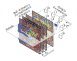
\includegraphics[width = 1\linewidth]{images/marco_teórico/diffractive_networks.png}
    \caption*{Fuente: Modificado de \textit{All-optical machine learning using diffractive deep neural networks, 2018.}}
    \label{fig:optical_networks}
\end{figure}

\section{CLASIFICACIÓN USANDO MEDIDAS CUADRÁTICAS}
En el campo de tomografía computarizada \myfootcite{douarre2020value} e imágenes de un solo píxel \myfootcite{bacca2020coupled}, se han propuesto sistemas de clasificación que usan únicamente medidas obtenidas a través de sistemas lineales de adquisición, debido al enfoque basado en el aprendizaje profundo en el que la arquitectura incluye una capa con el sistema óptico de adquisición. Asimismo, este enfoque ha sido estudiado en holografía \myfootcite{kim2018deep} y cristalografía de rayos-x \myfootcite{ziletti2018insightful}, donde las medidas obtenidas son difícilmente reconocidas por el ojo humano. 

Sin embargo, enfoques tradicionales de clasificación no han sido abordados en imágenes de medidas cuadráticas codificadas. Por lo tanto, este trabajo propone el desarrollo de un algoritmo de clasificación de objetos usando medidas cuadráticas codificadas bajo un enfoque de aprendizaje profundo. 




 % Marco de referencia
% ------------------------------------------------------------------------
% ------------------------------------------------------------------------
% ------------------------------------------------------------------------
%                                Capítulo 3
% ------------------------------------------------------------------------
% ------------------------------------------------------------------------
% ------------------------------------------------------------------------

\chapter{METODOLOGÍA PROPUESTA}

El enfoque de red neuronal profunda propuesto para la clasificación de objetos a partir de medidas cuadráticas codificadas incluye tres etapas principales: (i) capa de adquisición, (ii) enfoque de inicialización, (iii) y red de clasificación. La Figura \ref{fig:esquema_entrenamiento} ilustra el esquema de red neuronal profunda propuesto. Primero, una capa de adquisición simula el proceso de medición \eqref{eq:phase_retrieval_problem} a través del modelado de la propagación del campo óptico. Luego, un procedimiento de inicialización aproxima el campo óptico $\mathbf{z}$. Finalmente, la red de clasificación infiere la clase correspondiente a cada medida cuadrática codificada.


\begin{figure}[!h]
    \centering
    \caption{Esquema de red neuronal profunda de tres etapas propuesto para la clasificación de objetos a partir de medidas cuadráticas codificadas.}
    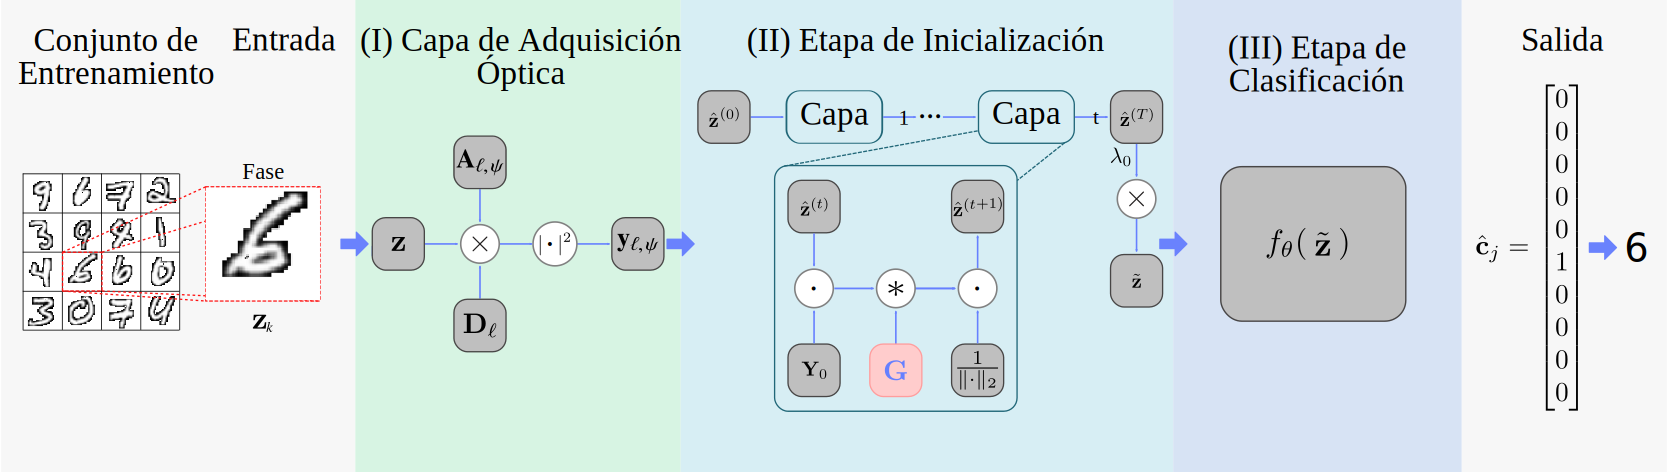
\includegraphics[width=\linewidth]{images/metodología/esquema_entrenamiento.pdf}
    \label{fig:esquema_entrenamiento}
\end{figure}


\section{ETAPA DE INICIALIZACIÓN}

En la etapa de inicialización del campo óptico, este trabajo aprovecha la matriz de adquisición $\mathbf{A}_{\ell, \psi}$ para crear un mapeo entre las medidas $\mathbf{y}_{\ell, \psi}$ y una aproximación más cercana del campo óptico $\mathbf{z}$, dada por el desenvolvimiento del algoritmo tradicional de inicialización de filtrado espectral \myfootcite{jerez2020fast} (FSI, de sus siglas en inglés \textit{filtered spectral initialization}), que incluye el aprendizaje de un filtro convolucional \myfootcite{Morales:22} (LFSI, de sus siglas en inglés \textit{learning filtered spectral initialization}), es decir que, $\hat{\mathbf{z}}=\mathrm{LFSI}(\mathbf{A}_{\ell, \psi}, \mathbf{y}_{\ell, \psi})$.

En concreto, este enfoque aplica un método iterativo para aproximar el campo óptico a partir de medidas cuadráticas codificadas, el cual se resume en el Algoritmo \ref{alg_1}. La aproximación dada por este algoritmo corresponde al cálculo de una versión filtrada de los mayores valores propios de la matriz
\begin{equation}
\mathbf{Y}_{0}:=\frac{1}{\mathrm{card}(\Xi)}\sum_{i\in\Xi}\frac{\mathbf{a}_{i,\psi}\mathbf{a}_{i,\psi}^\mathcal{H}}{\Vert\mathbf{a}_{i,\psi}\Vert_2^2},\label{eq:YO}
\end{equation}
donde $\mathbf{a}_{i,\psi}$ es la $i$-ésima columna de la matriz $\mathbf{A}=[\mathbf{A}_{1,\psi},\cdots,\mathbf{A}_{L,\psi}]^\mathcal{T}$, $\mathrm{card}(\cdot)$ es la cardinalidad del conjunto $\Xi$ correspondiente al conjunto de índices asignados a los valores más grandes de $\{(\mathbf{y})_i / \Vert \mathbf{a}_{i,\psi}\Vert_{2}\}$ con $\mathbf{y}=[\mathbf{y}_{1,\psi}^\mathcal{T},\cdots,\mathbf{y}_{L,\psi}^\mathcal{T}]^\mathcal{T}$.  Encontrar $\tilde{\mathbf{z}}$, teniendo en cuenta $\mathbf{Y}_0$ es posible resolviendo el siguiente problema de optimización


\begin{equation}
    \tilde{\mathbf{z}}=\argmax_{\Vert{\mathbf{z}}\Vert_2=1}{\mathbf{z}}^\mathcal{H}\mathbf{Y}_{0}{\mathbf{z}}.
\end{equation}


Tenga en cuenta que, la matriz $\mathbf{Y}_{0}$ se calcula en la línea 4 del Algoritmo \ref{alg_1}. En la línea 6, se aplica el filtrado mediante la operación de convolución $*$ entre $\mathbf{Y}_{0}\hat{\mathbf{z}}^{(t)}$ y en el kernel $\mathbf{G}$. Luego, la aproximación filtrada se normaliza en la línea 7. Finalmente, este algoritmo devuelve el vector complejo $\tilde{\mathbf{z}}$ en la línea 10, que se multiplica por el factor de escala $\lambda_0=\sqrt{\sum_{\ell=1}^{L}\frac{\Vert\mathbf{y}_{\ell,\psi}\Vert_{2}^2}{nL}}$ . %\textcolor{negro}{$\mathcal{O}(n\log n)$ }
  

Este trabajó propone la inicialización aprendida realizando un desenvolvimiento del algoritmo FSI en un esquema de red neuronal, como se muestra en la Figura \ref{fig:esquema_entrenamiento}. Adicionalmente, se incluye el filtro $\mathbf{G}$ como un parámetro entrenable de la red neuronal bajo una regularización definida a través de la siguiente función indicadora
\begin{equation}
  \mathcal{I}_{\Omega}(\mathbf{G})=  \left\{\begin{matrix}
 0& \text{si } \mathbf{G}\in \Omega \\ 
+\infty & \text{si } \mathbf{G}\notin \Omega 
\end{matrix}\right., \label{eq:regularizationG}
\end{equation}
donde $\Omega=\{\mathbf{G}\in\mathbb{C}^{g\times g}| |(\mathbf{G})_{p,q}|\leq 1\}$. 


\begin{algoritmo}[!h]
    %\scriptsize
    \caption{Algoritmo LFSI }\label{fsi_algo}
    \begin{algorithmic}[1]
        \State{\textbf{Entrada:} Matriz de sensado y muestras $\{(\mathbf{A}_{\ell,\psi};\mathbf{y}_{\ell,\psi})\}_{\ell=1}^L$, máximo número de iteraciones $T$, filtro $ \mathbf{G}\in\mathbb{C}^{g\times g}$.}
		\State{$\hat{\mathbf{z}}\leftarrow$ Escogido aleatoriamente.}
		\State{\textbf{Asignar }$\Xi$ como el conjunto de índices correspondientes a los valores más grandes de $\{(\mathbf{y})_i / \Vert \mathbf{a}_{i,\psi}\Vert_{2}\}$.}
		\State{$$\mathbf{Y}_{0}:=\frac{1}{\mathrm{card}(\Xi_0)}\sum_{i\in\Xi}\frac{\mathbf{a}_{i,\psi}\mathbf{a}_{i,\psi}^\mathcal{H}}{\Vert\mathbf{a}_{i,\psi}\Vert_2^2}$$}
		\For{$t=0:T-1$} 
		\State{$\grave{\mathbf{z}}^{(t+1)}= \mathbf{G}*\left(\mathbf{Y}_{0}\hat{\mathbf{z}}^{(t)}\right).$\Comment{Filtrado}}
		\State{$\hat{\mathbf{z}}^{(t+1)}=\frac{\grave{\mathbf{z}}^{(t+1)}}{\left \| \grave{\mathbf{z}}^{(t+1)} \right \|_2}$}.		\Comment{Normalización}
		\EndFor
		\State{Compute $\tilde{\mathbf{z}} = \lambda_0\hat{\mathbf{z}}^{(T)}$.\Comment{Escalado}}
		%		\State{Compute $\mathbf{z}_{1}=\mathcal{A}(\mathbf{z}_{0})$\Comment{Denoising step}}
		\State{\textbf{salida: } Estimación inicial del campo óptico $\tilde{\mathbf{z}}$.}
	\end{algorithmic}
    \label{alg_1}
\end{algoritmo}


\section{ETAPA DE CLASIFICACIÓN}

En este trabajo, se propone un esquema de clasificación de medidas cuadráticas codificadas. Para realizar la tarea de clasificación se puede usar diferentes modelos de clasificación, en este sentido, se utilizaron tres arquitecturas de clasificación del estado del arte: MobilNetV2 \myfootcite{mobilnetv2}, InceptionV3 \myfootcite{inceptionv3}  y Xception \myfootcite{xception}. La Tabla \ref{tab:comp_class_models} resume una el número de parámetros, la cantidad de capas y la profundidad de las arquitecturas de redes neuronales empleadas.

\begin{table}[!h]
\centering
\caption{Resumen de las arquitecturas de redes neuronales de clasificación utilizadas.}
\begin{tabular}{|c|c|c|}
\hline
\textbf{Modelo}      & \textbf{Número de parámetros} & \textbf{Número de capas} \\ \hline
MobileNetV2 & 3,538,984            & 53              \\ \hline
InceptionV3 & 23,851,784           & 48              \\ \hline
Xception    & 22,910,480           & 71              \\ \hline
\end{tabular}
\label{tab:comp_class_models}
\end{table}

El entrenamiento de los pesos $\theta$ de la red de clasificación $f_\theta(\cdot)$, se realizó mediante el siguiente problema de optimización

\begin{equation}
    \mathbf{\theta}^* \in  \argmin_{\mathbf{\theta}} \frac{1}{K}\sum_{k = 1}^{K} \mathcal{L}\left( c^{(k)}, f_\theta(\mathrm{LFSI}\left(\mathbf{A}_{\ell,\psi},\mathbf{y}_{\ell, \psi}\right)\right).
    \label{eq:dl_optimization}
\end{equation}

Este problema minimiza la función pérdida usualmente conocida como entropía categórica cruzada $\mathcal{L}(\cdot, \cdot)$ entre las etiquetas del conjunto de datos $c^{(k)}$, y las clases predichas $\hat{c}^{(k)} = f_\theta(\mathrm{LFSI}\left(\mathbf{A}_{\ell,\psi},\mathbf{y}_{\ell, \psi}\right))$, donde $K$ es el número total de ejemplos del conjunto de datos, $\mathbf{y}_{\ell, \psi}^{(k)}$ es la medida cuadrática codificada del $k$-ésimo ejemplo.


\section{ESQUEMA PROPUESTO DE CLASIFICACIÓN DE OBJETOS}

El Algoritmo \ref{alg:algoritmo_2} resume el proceso de entrenamiento del esquema mostrado en la Figura \ref{fig:esquema_entrenamiento}. En primer lugar, en la línea 2, el filtro es inicializado usando una distribución uniforme $\mathcal{U}(\mathbf{0},\mathbf{1})$. Luego, el modelo de propagación descrito por \eqref{eq:phase_retrieval_problem} es simulado por la capa de adquisición en la línea 5. Posteriormente, en línea 6, se realiza el proceso de inicialización que aproxima el campo óptico inicial con base en las medidas cuadráticas codificadas obtenidas. En las líneas 7-9, el optimizador Adam $\mathcal{A}_{dam}(\cdot)$ se implementa para minimizar la función de pérdida \eqref{eq:dl_optimization} entre la clase etiquetada en el conjuto de datos ${\mathbf{c}}^{(k)}$ y la predicción $f_{\boldsymbol{\theta}}\left(\tilde{\mathbf{z}}^{(k)}\right)$. Esta función se minimiza sobre el filtro de la inicialización y los parámetros de la red neuronal de clasificación ponderados por $\beta_1$ y $\beta_2$, respectivamente. Finalmente, estos parámetros óptimos $\mathbf{G}$ y $\boldsymbol{\theta}$ se devuelven en la línea 12.


\begin{algoritmo}[!h]

        \caption{Enfoque de clasificación de objetos.}
            \label{alg:algoritmo_2}
        	\begin{algorithmic}[1]
            \State{\textbf{Entrada:} Conjunto de entrenamiento $\{\mathbf{z}^{(k)}, {\mathbf{c}}^{(k)}\}_{k=1}^\mathcal{K}$ con $\mathcal{K}$ imágenes.}  
            \State{\textbf{Inicialización filtro:} {\small
            $\mathbf{G}\in \mathcal{U}(\mathbf{0},\mathbf{1})^{5 \times 5}$} }
            \For{época = 1:$\mathcal{E}$}\Comment{$\mathcal{E}$ épocas}
                \For{$k= 1$:$\mathcal{K}$}\Comment{$\mathcal{K}$ ejemplos}
                    \State{$\mathbf{y}_{\ell,\psi} = \vert \mathbf{A}_{\ell,\psi}\mathbf{z}^{(k)}\vert^2, \quad \ell\in\{1,\dots,L\}$}
                    \Comment{Médidas cuadráticas codificadas}
                    \State{$\tilde{\mathbf{z}}^{(k)} \leftarrow  { \mathrm{LFSI}\left(\mathbf{A}_{\ell,\psi},\mathbf{y}_{\ell, \psi}\right)}$}\Comment{Algoritmo \ref{alg_1}}
                    %\State{$\hat{\mathbf{c}}^{(k)} \leftarrow  f_{\boldsymbol{\theta}}\left(\tilde{\mathbf{z}}^{(k)}\right)$}\Comment{Bloque de clasificación}
                    \State{$\mathcal{L}_{\mathbf{G},\boldsymbol{\theta}}=\frac{1}{\mathcal{K}}\sum_{k=1}^{\mathcal{K}} \mathcal{L}\left( c^{(k)},f_{\boldsymbol{\theta}}\left(\tilde{\mathbf{z}}^{(k)}\right) \right) $}    
               \Comment{Función de costo}     
                    \State{$\mathbf{G}\leftarrow\mathcal{A}_{dam}( \mathbf{G}, \beta_1 \nabla_{\mathbf{G}} \mathcal{L}_{\mathbf{G},\boldsymbol{\theta}}) $}    
                \Comment{Optimización sobre $\mathbf{G}$ }
                      \State{$\boldsymbol{\theta}\leftarrow\mathcal{A}_{dam}( \boldsymbol{\theta}, \beta_2 \nabla_{\boldsymbol{\theta}} \mathcal{L}_{\mathbf{G},\boldsymbol{\theta}}) $}    
                \Comment{Optimización sobre $\boldsymbol{\theta}$ }
                \EndFor
                \EndFor
		\State{\textbf{Salida: } Kernel óptimo $\mathbf{G}$ y parámetros de la red neuronal $\boldsymbol{\theta}$.}
	\end{algorithmic}
	%\label{alg:algoritmo_2}
\end{algoritmo}
 % Modelo matemático del DRON
% ------------------------------------------------------------------------
% ------------------------------------------------------------------------
% ------------------------------------------------------------------------
%                                Capítulo 4
% ------------------------------------------------------------------------
% ------------------------------------------------------------------------
% ------------------------------------------------------------------------

\chapter{SIMULACIONES Y RESULTADOS}

En esta sección se presentan los resultados obtenidos a partir del método propuesto para la clasificación de objetos basado en medidas medidas cuadráticas codificadas y su comparación con esquemas de clasificación del estado del arte.

\section{CONJUNTO DE DATOS}

Durante el desarrollo de este trabajo, no se encontraron conjuntos de datos públicos enfocados en la clasificación de medidas cuadráticas. Debido a esto, se decidió simular la propagación de las medidas usando conjuntos de datos tradicionales. Para este fin se usaron imágenes de los conjuntos de datos MNIST \myfootcite{deng2012mnist} y Fashion-MNIST \myfootcite{xiao2017fashion}. Por un lado, la Figura \ref{fig:conjunto_datos} muestra un ejemplo de las imágenes presentes en los conjuntos de datos usados. Por otro lado, el Cuadro \ref{tab:conjunto_datos} muestra la división de datos en entrenamiento, validación y prueba. Cada imagen fue escalada en el rango de $[-\pi, \pi]$ y usada como información de fase de la forma $\mathbf{z}=e^{j\mathrm{ang}(\mathbf{z})}$.

\begin{figure}[!h]
    \centering
    \caption{Ejemplo de las imágenes presentes en los conjuntos de datos MNIST y Fashion-MNIST.}
    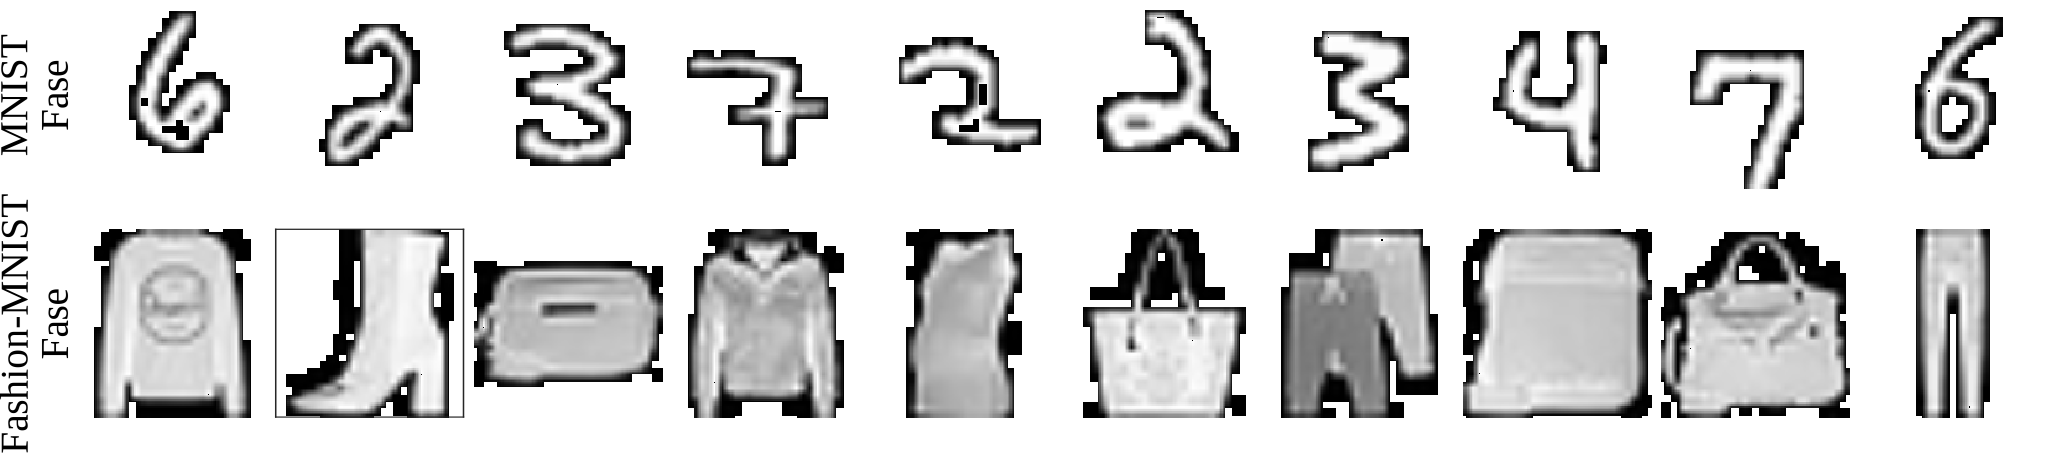
\includegraphics[width=\linewidth]{images/resultados/datasets.pdf}
    \label{fig:conjunto_datos}
\end{figure}


% Please add the following required packages to your document preamble:
% \usepackage{graphicx}
\begin{table}[!h]
\caption{Resumen de la división de los conjuntos de datos usados para evaluar el método propuesto.}
\centering\scalebox{0.9}{
\resizebox{\textwidth}{!}{%
\begin{tabular}{|c|c|c|c|c|}
\hline
\textbf{Conjunto de datos} & \textbf{Entrenamiento} & \textbf{Validación} & \textbf{Prueba} & \textbf{Total} \\ \hline
MNIST                      & 54000                  & 6000                & 10000           & 70000          \\ \hline
Fashion-MNIST              & 54000                  & 6000                & 10000           & 70000          \\ \hline
\end{tabular}%
}}
\label{tab:conjunto_datos}
\end{table}

\section{MÉTRICAS}
La calidad de la inicialización y la precisión de la clasificación en sistemas de difracción basados en medidas cuadráticas codificadas, se mide a través de las siguientes métricas.
\subsection{Métricas para evaluar la inicialización.}

A continuación, se describen las métricas usadas para evaluar la estimación inicial $\hat{\mathbf{z}}$ respecto a la imagen de referencia $\mathbf{z}$.
\begin{itemize}
    \item Medida del índice de similitud estructural (SSIM):
    
    \begin{equation}
        %\nonumber
        \mathrm{SSIM}(\mathbf{z}, \tilde{\mathbf{z}}) = \frac{2(\mu_{\mathbf{z}}\mu_{\tilde{\mathbf{z}}} + C_1) + (2\sigma_{\mathbf{z}\tilde{\mathbf{z}}} + C_2)}{(\mu_{\mathbf{z}} + \mu_{\tilde{\mathbf{z}}} + C_1)(\sigma_{\mathbf{z}}\sigma_{\tilde{\mathbf{z}}} + C_1)},
        \label{eq:SSIM}
    \end{equation}
    
    donde $(\mu_{\mathbf{z}}, \sigma_{{\mathbf{z}}})$ y $(\mu_{\tilde{\mathbf{z}}}, \sigma_{\tilde{\mathbf{z}}})$ representan la media y la varianza de ${\mathbf{z}}$ y $\tilde{\mathbf{z}}$ respectivamente, además $\sigma_{\mathbf{z}\tilde{\mathbf{z}}}$ es la covarianza entre ellos. Por último, $C_1 = (k_1L)^2$ y $C_2 = (k_2L)^2$ son dos constantes para prevenir división por cero y $k_1 = 0.01$ y $k_2 = 0.03$. Esta métrica tiene valores en el rango de $[0, 1]$, es decir, a mayor valor, mejor es la estimación.
    
    \item Relación de señal a ruido máxima (PSNR):
    \begin{equation}
        %\nonumber
        \mathrm{PSNR}(\mathbf{z}, \tilde{\mathbf{z}})=10 \cdot \log_{10}\left(\frac{\mathrm{MAX}^{2}}{\mathrm{MSE}(\mathbf{z}, \tilde{\mathbf{z}})}\right),
        \label{eq:PSNR}
    \end{equation}
    donde $\mathrm{MAX}(\cdot)$ es el rango dinámico de la imagen y $\mathrm{MSE}(\cdot)$ es el error cuadrático medio entre la imagen original y la estimación. Esta métrica tiene valores en el rango de $[0, \infty)$, es decir, a mayor valor, mejor es la estimación.
    
    \item Error cuadrático medio (MSE):
    
    \begin{equation}
        %\nonumber
        \mathrm{MSE}(\mathbf{z}, \tilde{\mathbf{z}}) = \frac{1}{n} \Vert \mathbf{z} - \tilde{\mathbf{z}}\Vert_2^2.
        \label{eq:MSE}
    \end{equation}
    
    Esta métrica tiene valores en el rango de $[0, \infty)$, es decir, a menor valor, mejor es la estimación.

    \item Error relativo (RE): 
    \begin{equation}
        %\nonumber
        \mathrm{RE}(\mathbf{z}, \tilde{\mathbf{z}}) = \frac{ \mathrm{dist}(\mathbf{z}, \hat{\mathbf{z}})}{\Vert \mathbf{z} \Vert_2}.
        \label{eq:RE}
    \end{equation}
    
    Esta métrica tiene valores en el rango de $[0, \infty)$, donde a menor valor, mejor es la estimación.
\end{itemize}
\subsection{Métricas para evaluar la clasificación.}
Las métricas usadas para evaluar la clasificación se presentan a continuación, donde los valores a calcular dependen de los verdaderos positivos $TP$, verdaderos negativos $TN$, falsos positivos $FP$, y falsos negativos $FN$, asociados a la clase de cada ejemplo del conjunto de datos.


\begin{itemize}
    \item Exactitud: esta medida corresponde a la proporción de predicciones predichas correctamente,

    \begin{equation}
        \mathrm{Exactitud}= \frac{TP+TN}{TP+TN+FP+FN}.
        \label{eq:acc}
    \end{equation}


    \item Precisión: esta medida es la proporción de ejemplos pertenecientes a una clase que fueron correctamente predichos en dicha clase,
    
        \begin{equation}
            \mathrm{Precisión} = \frac{TP}{TP+FP}.
            \label{eq:pre}
        \end{equation}
        
    \item Exhaustividad: esta medida es la proporción entre las predicciones que fueron correctamente clasificadas en una clase sobre los ejemplos que pertenecían a esa clase,
    
    \begin{equation}
        \mathrm{Exhaustividad}= \frac{TP}{TP+FN}.
        \label{eq:re}
    \end{equation}

    \item Métrica-F1: esta medida está diseñada para ponderar de manera equilibrada entre las métricas de precisión (\ref{eq:pre}) y exhaustividad (\ref{eq:re}),
    
    \begin{equation}
        \mathrm{F1} = \frac{2\cdot\mathrm{Precisión}\cdot\mathrm{Exhaustividad}}{\mathrm{Precisión}+\mathrm{Exhaustividad}}.
        \label{eq:f1}
    \end{equation}

\end{itemize}

\section{EXPERIMENTOS}

% \subsection{Métodos de Comparación}

% \begin{itemize}
%     \item Comparación estimación inicial.
    
%     Estimar el campo óptico inicial es una tarea ampliamente estudiada en el estado del arte de recuperación de la fase. Específicamente resaltan métodos tales como el propuesto \myfootcite{Morales:22}, \textit{orthogonality-promoting initialization} (OPI) \myfootcite{wang2017solving}, \textit{weighted maximal correlation initialization} (WMCI) \myfootcite{wang2018phase}, y \textit{filtered spectral initialization} (FSI) \myfootcite{jerez2020fast}. Estos métodos de estimación inicial son usados como etapa inicial por algoritmos de reconstrucción tales como TWF, TAF y RAF.
    
    
%     \item Comparación clasificación.
    
%     Para comparar el método propuesto se encontró que el esquema tradicional de clasificación sobre medidas cuadráticas se realiza como se muestra en la Figura \ref{fig:esquema_entrenamiento_tradicional}
    
%     \begin{minipage}[!h]{\linewidth}
      
%       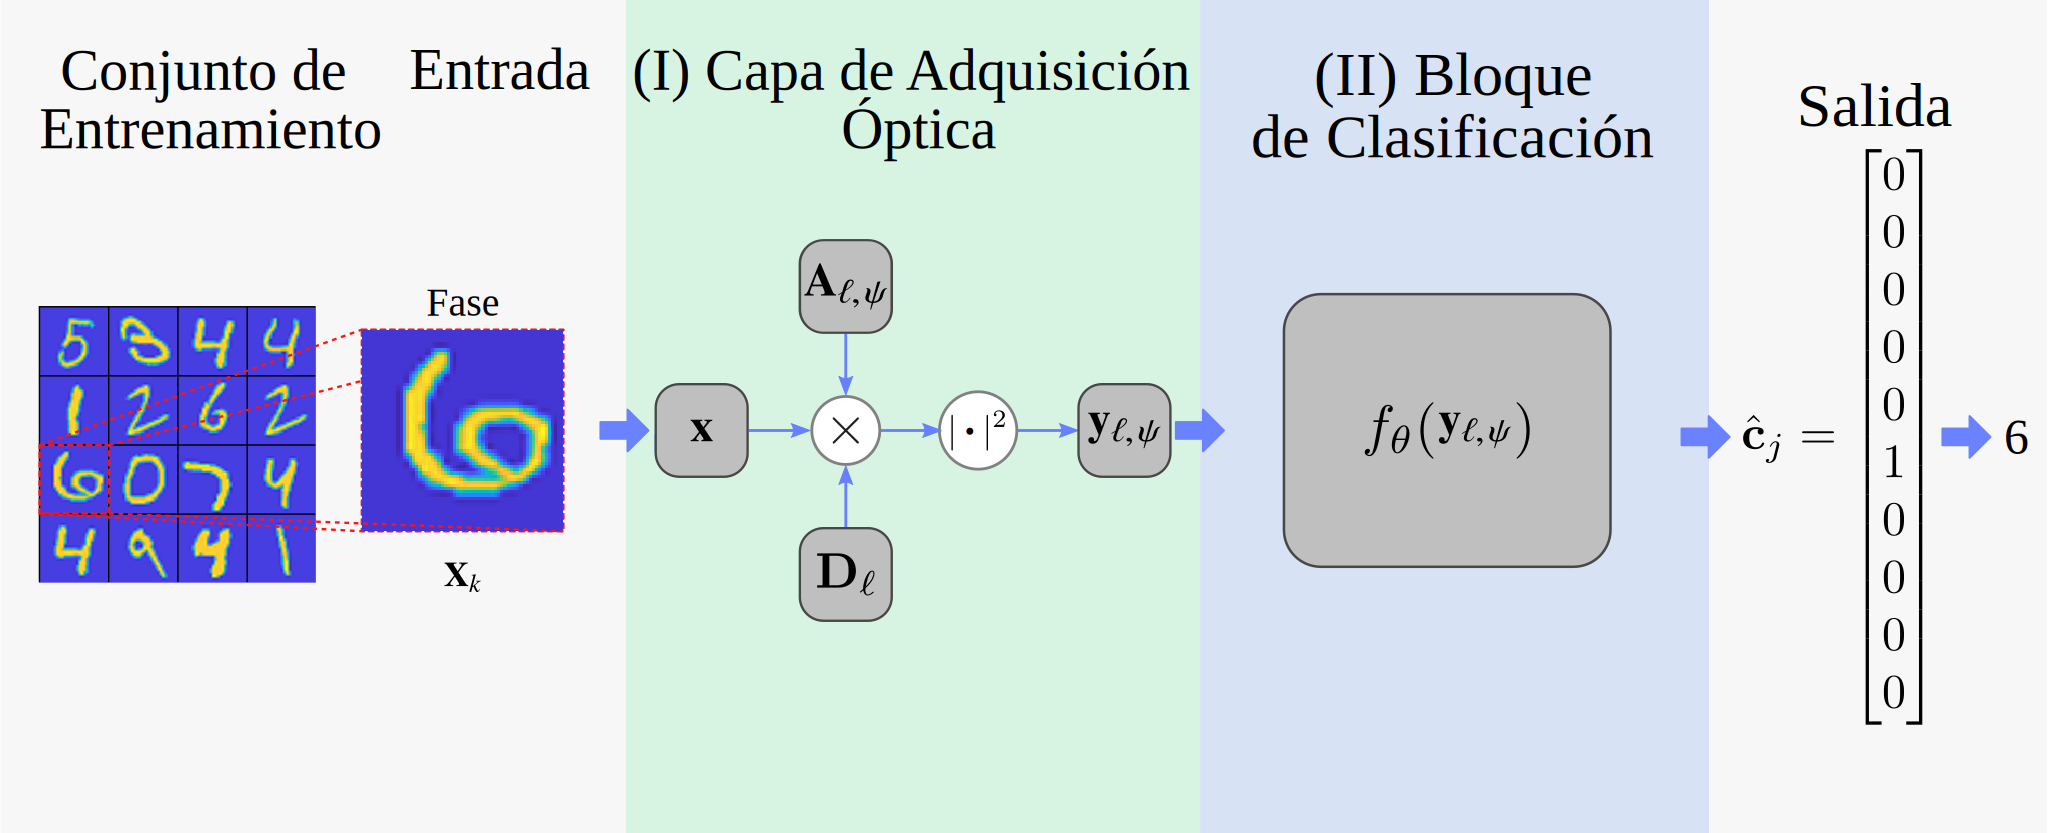
\includegraphics[width=\linewidth]{images/metodología/esquema_entrenamiento_tradicional.pdf}
%       \captionof{figure}{Esquema de clasificación usado en el estado del arte.}
%         \label{fig:esquema_entrenamiento_tradicional}
%     \end{minipage}
    
%     En el esquema tradicional no se realiza una modulación del campo óptico, por lo tanto para la comparación con el estado del arte la codificación corresponde a $\mathbf{D}_\ell = 1$.
    
%     Adicionalmente se realizó la comparación haciendo uso del operador inverso de la propagación del campo óptico $\mathcal{P}_{\ell, \psi}:\mathbb{C}^n\rightarrow \mathbb{C}^n$ para estimar $\hat{\mathbf{x}}$ \myfootcite{katkovnik2017computational},
    
%     \begin{equation}
%         \hat{\mathbf{x}}= \frac{1}{L}\sum_{\ell=1}^{ L} \mathcal{P}_{\ell, \psi}(\mathbf{y}_{\ell, \psi}).
%         \label{eq:back_propagation}
%     \end{equation}
% \end{itemize}

\subsection{Configuración experimental.}

En esta subsección, se presentan los parámetros de simulación utilizados para el modelo de propagación, la etapa de inicialización y la red neuronal de clasificación. Todos los experimentos realizados en este trabajo fueron implementados en \textit{Python 3.9} usando la herramienta \textit{Tensorflow 2.4.1}  \myfootcite{tensorflow2015-whitepaper}. Los experimentos se ejecutaron sobre un computador con GPU Nvidia 3090 RTX con 64 Gb de memoria RAM y CPU Intel(R) Xeon(R) W-3223 CPU @ 3.50GHz. El código usado para los experimentos de este trabajo puede ser consultado de manera pública en \footnote{\href{https://github.com/David-Morales-Norato/code_undergrad_thesis}{https://github.com/David-Morales-Norato/code\_undergrad\_thesis}}. En relación con los parámetros de propagación, el Cuadro \ref{tab:parameters} presenta los parámetros ópticos fijados para calcular la matriz $\mathbf{A}_{\ell,\psi}$ definida en \eqref{eq:phase_retrieval_problem} según cada campo de difracción. Estos parámetros permiten simular la adquisición de las medidas cuadráticas codificadas a lo largo de cada campo de difracción usando la capa de adquisición óptica. En la etapa de inicialización, el filtro $\mathbf{G} \in \mathbb{C}^{g\times g}$ entrenable fue fijado a un tamaño de kernel $g=5$ y un número de iteraciones $T=10$. La estimación del campo óptico inicial es una tarea ampliamente estudiada en el estado del arte de recuperación de la fase. Específicamente, se destacan métodos de inicialización, tales como \textit{orthogonality-promoting initialization} (OPI) \myfootcite{wang2017solving}, \textit{weighted maximal correlation initialization} (WMCI) \myfootcite{wang2018phase}, y FSI \myfootcite{jerez2020fast}. Cabe señalar que, estos métodos de inicialización fueron usados para comparar la inicialización propuesta LFSI, donde se comparó la robustez al ruido, el número de iteraciones ${T}$ y el número de proyecciones ${L}$ requeridas para lograr una estimación apropiada. 

Finalmente, para realizar la clasificación se usaron las arquitecturas MobilNetV2 \myfootcite{mobilnetv2}, InceptionV3 \myfootcite{inceptionv3} y Xception \myfootcite{xception}, las cuales fueron entrenadas usando una tasa de aprendizaje de $1\times 10^{-3}$ con el algoritmo de optimización Adam a partir de $\mathcal{E}=100$ épocas para entrenar los conjuntos de datos MNIST y Fashion-MNIST. Para comparar el esquema de clasificación propuesto se implementó el esquema de clasificación tradicional \myfootcite{kim2018deep}$^,$\myfootcite{ ziletti2018insightful}, donde se realiza únicamente el proceso de simulación de las medidas cuadráticas sin el proceso de estimación del campo óptico. Asimismo, se empleó el método propuesto de filtrado espectral aprendido en las Figuras \ref{fig:results_mob}, \ref{fig:results_inc} y \ref{fig:results_xce}. Por otra parte, se reemplazó en la etapa de inicialización del esquema de clasificación propuesto, el algoritmo de inicialización LFSI por el modelo de propagación inverso (BPM, de sus siglas en inglés \textit{back-propagation matrix}) $\mathbf{A}_{\ell, \psi}^{-1}$ para obtener una estimación rápida del campo óptico inicial, como se presenta en las Figuras \ref{fig:results_mob}, \ref{fig:results_inc} y  \ref{fig:results_xce}. Esta estimación rápida está dada por 

\begin{equation}
    \hat{\mathbf{z}}= \frac{1}{L}\sum_{\ell=1}^{ L} \mathbf{A}_{\ell, \psi}^{-1}\mathbf{y}_{\ell, \psi}
    \label{eq:back_propagation}.
\end{equation}

Es importante señalar que, $\mathbf{z} \neq \mathbf{A}_{\ell, \psi}^{-1}\mathbf{y}_{\ell}$, debido a la pérdida de la información de fase que induce el operador de magnitud $\vert \cdot \vert$ presente en el modelo de propagación \eqref{eq:phase_retrieval_problem}.


% Por último, todos los experimentos realizados en este trabajo fueron implementados en \textit{Python 3.9} usando la herramienta \textit{Tensorflow 2.4.1}  \myfootcite{tensorflow2015-whitepaper}. Los experimentos se ejecutaron sobre un computador con GPU Nvidia 3090 RTX con 64 Gb de memoria RAM y CPU Intel(R) Xeon(R) W-3223 CPU @ 3.50GHz. El código usado para los experimentos de este trabajo puede ser consultado de manera pública en el siguiente enlace: \href{https://github.com/David-Morales-Norato/code_undergrad_thesis}{https://github.com/David-Morales-Norato/code\_undergrad\_thesis}

\begin{table}[!h]
\centering
\caption{ Parámetros de propagación usados para simular el modelo de propagación \eqref{eq:phase_retrieval_problem} para cada campo de difracción.}
\scalebox{0.9}{
\begin{tabular}{|l|r|r|c|}
\hline
\multicolumn{1}{|c|}{\textbf{Parámetros ópticos}} & \multicolumn{1}{c|}{\textbf{Campo cercano}} & \multicolumn{1}{c|}{\textbf{Campo medio}} & \textbf{Campo lejano} \\ \hline
Longitud de onda ($\lambda$) [nm]                    & 635                           & 635                            & -         \\ \hline
Distancia de propagación ($z$) [cm]         &    2.5                       & 7                              & -         \\ \hline
\end{tabular}}
\label{tab:parameters}
\end{table}


\subsection{Resultados de la inicialización.}


La Figura \ref{fig:results_initializations} muestra el desempeño en la métrica de RE del método de estimación inicial propuesto comparando con los algoritmos FSI, OPI y WMCI variando el número de iteraciones $T$ para los conjuntos de datos MNIST y Fashion-MNIST en los tres campos de difracción cercano, medio y lejano, donde se puede observar que el método propuesto logra superar los métodos tradicionales obteniendo una estimación inicial apropiada a partir de un número menor de iteraciones.

\begin{figure}[!h]
\centering
    \caption{Resumen del desempeño de la inicialización propuesta comparando con los métodos FSI, OPI, WMCI sobre la métrica de RE, variando el número de iteraciones del algoritmo para estimar imágenes de los conjuntos MNIST y Fashion-MNIST en los campos de difracción cercano, medio y lejano.}
    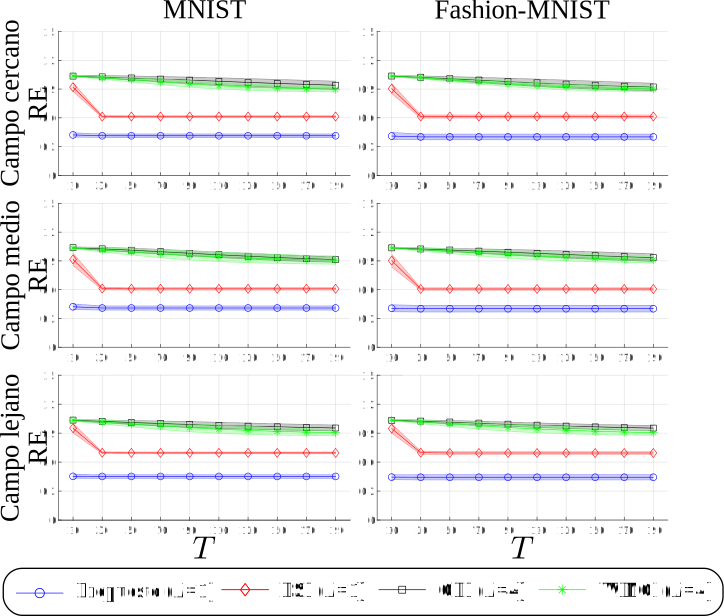
\includegraphics[width=0.85\linewidth]{images/resultados/results_initializations.pdf}
        \label{fig:results_initializations}
\end{figure}



La Figura \ref{fig:noisy_scenario} muestra la evaluación de la robustez del método frente al ruido. En este caso, se adicionó ruido aditivo gaussiano con $\mathrm{SNR} = 10, 15$ y $30$ dB. Cabe resaltar que, el método propuesto muestra una mayor estabilidad al ruido comparando con los métodos de inicialización del estado del arte.

\begin{figure}[!h]
    \caption{Resumen del desempeño de la inicialización comparando con diferentes estrategias del estado del arte. Se varió el número de medidas $T$ para realizar la estimación y diferentes niveles de ruido afectando las medidas descritos por el SNR.}
    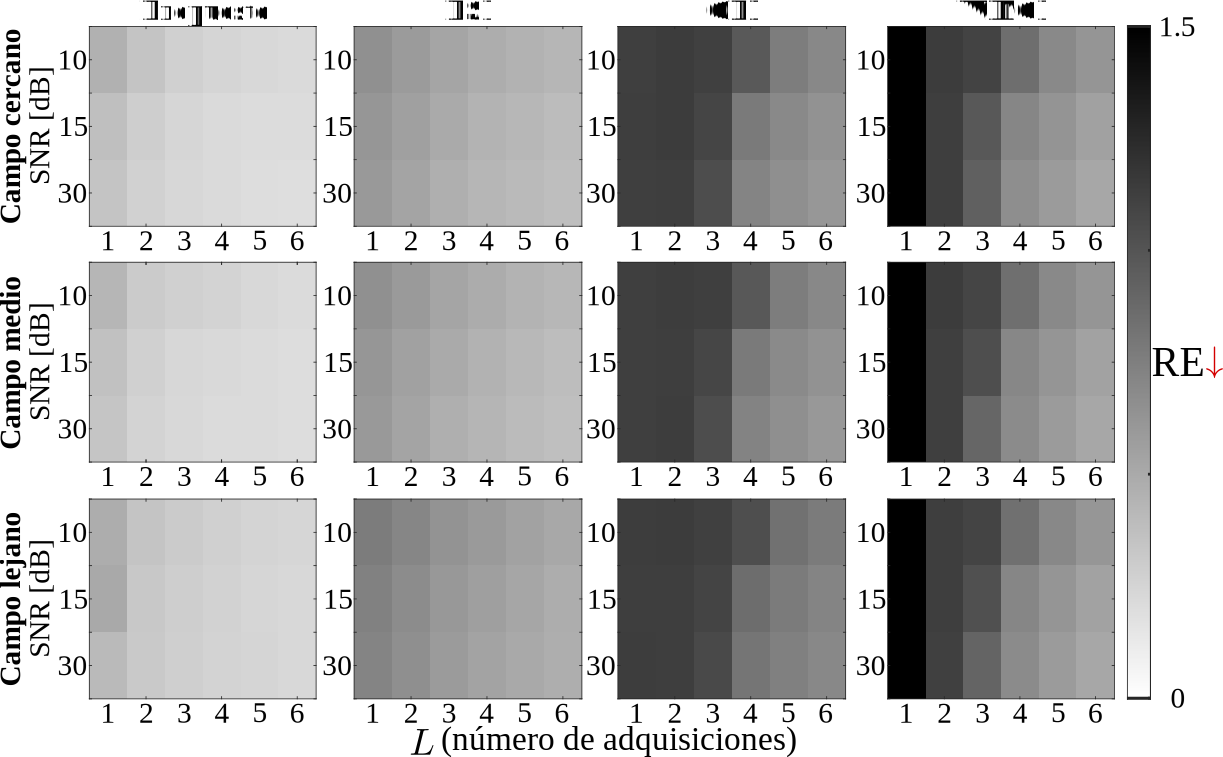
\includegraphics[width=1\linewidth]{images/resultados/Noisy_Initializations.pdf}
    \label{fig:noisy_scenario}
\end{figure}

Por último, la Figura \ref{fig:resultados_inicialización_sin_ruido} presenta los resultados visuales de la estimación del campo inicial, donde se observa en escala de grises la fase de cada estimación para el conjunto de datos MNIST y Fashion-MNIST. Para comparar el método propuesto se implementaron los algoritmos FSI con $L = 1, T = 10$, FSI usando $L = 1, T=200$, OPI $L = 4, T=200$ y WMCI $L = 4, T=200$. Se puede observar que, el método propuesto logra aproximar el campo óptico en los tres campos de difracción simulados a un bajo número de iteraciones utilizando una única proyección $L=1$ y $T=10$ número de iteraciones.

\begin{figure}[!h]
    \centering
    \caption{Resultados visuales de la estimación del campo óptico inicial comparando el método propuesto contra el algoritmo FSI con $L = 1, T = 10$, FSI usando $L = 1, T=200$, OPI $L = 4, T=200$ y WMCI $L = 4, T=200$.}
    \includegraphics[width=\linewidth]{images/resultados/resultados_inicialización_sin_ruido.pdf}
    \label{fig:resultados_inicialización_sin_ruido}
\end{figure}

\pagebreak

\subsection{Resultados de la clasificación de objetos.}

Los resultados de los experimentos de clasificación se resumen a continuación. Las Figuras \ref{fig:results_mob}, \ref{fig:results_inc} y \ref{fig:results_xce} exhiben los resultados del desempeño de la clasificación de medidas cuadráticas codificadas en términos de las métricas de exactitud, precisión, exhaustividad y F1 utilizando las redes de clasificación MobilNetV2 en la Figura \ref{fig:results_mob}, InceptionV3 en la Figura \ref{fig:results_inc} y Xception en la Figura \ref{fig:results_xce}. Cada figura representa la comparación de los esquemas de clasificación tradicional, y los métodos propuestos BPM y LFSI. La clasificación se realizó sobre medidas simuladas en los campos de difracción cercano, medio y lejano. Es importante resaltar que, el método tradicional muestra un desempeño menor en todas las métricas comparando con los métodos propuestos BPM y LFSI para cada uno de los campos de difracción y redes de clasificación.

Específicamente, el método propuesto supera al método tradicional en hasta 0.24, 0.2, 0.25 y 0.22 en términos de exactitud, precisión, exhaustividad y métrica F1, respectivamente. En particular, estas ganancias se reportan para la clasificación de objetos utilizando medidas simuladas del campo lejano a partir del conjunto de datos de Fashion-MNIST. En el caso del campo medio, se supera en 0.21, 0.13, 0.21, y 0.17 y para el campo cercano, se supera en 0.1, 0.14, 0.13, y 0.14 en exactitud, en precisión, en exhaustividad y en F1, respectivamente. 

\begin{figure}[!h]
    \centering
    \caption{Resultados en la métrica de exactitud, precisión, exhaustividad y F1 para evaluar la clasificación de medidas cuadráticas codificadas simuladas sobre el campo cercano, medio y lejano. Se muestra la comparación de la clasificación Tradicional, el uso del propagador inverso propuesto (BPM) y el método de inicialización aprendida (LFSI) usando la arquitectura MobilNetV2, sobre la división de prueba de los conjuntos de datos MNIST y Fashion-MNIST.}
    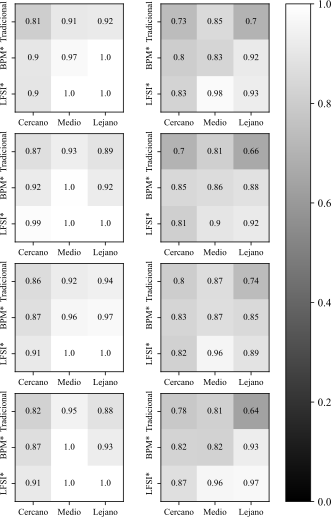
\includegraphics[height=0.8\textheight]{images/resultados/test_result_mobilnet.pdf}
    \label{fig:results_mob}
\end{figure}


\begin{figure}[!h]
    \centering
    \caption{Resultados en la métrica de exactitud, precisión, exhaustividad y F1 para evaluar la clasificación de medidas cuadráticas codificadas simuladas sobre el campo cercano, medio y lejano. Se muestra la comparación de la clasificación Tradicional, el uso del propagador inverso propuesto (BPM) y el método de inicialización aprendida (LFSI) usando la arquitectura InveptionV3, sobre la división de prueba de los conjuntos de datos MNIST y Fashion-MNIST.}
    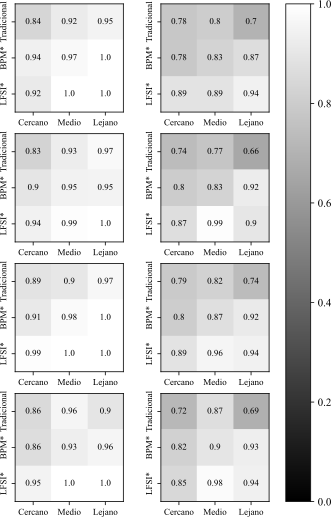
\includegraphics[height=0.8\textheight]{images/resultados/test_result_inception.pdf}
    \label{fig:results_inc}
\end{figure}

\begin{figure}[!h]
    \centering
    \caption{Resultados en la métrica de exactitud, precisión, exhaustividad y F1 para evaluar la clasificación de medidas cuadráticas codificadas simuladas sobre el campo cercano, medio y lejano. Se muestra la comparación de la clasificación Tradicional, el uso del propagador inverso propuesto (BPM) y el método de inicialización aprendida (LFSI) usando la arquitectura Xception, sobre la división de prueba de los conjuntos de datos MNIST y Fashion-MNIST.}
    \includegraphics[height=0.8\textheight]{images/resultados/test_result_xception.pdf}
    \label{fig:results_xce}
\end{figure}
 % Controladores PI y su conjunto estabilizante
% \input{Secs/T5} % Recomendaciones
% ------------------------------------------------------------------------
% ------------------------------------------------------------------------
% ------------------------------------------------------------------------
%                            Trabajo futuro
% ------------------------------------------------------------------------
% ------------------------------------------------------------------------
% ------------------------------------------------------------------------

\chapter{TRABAJO FUTURO}
% ------------------------------------------------------------------------
% \noindent Actividades complementarias a los desarrollos presentados, incluyen el cálculo automático para conjuntos estabilizantes en plantas arbitrarias empleando el \emph{método de la signatura} desarrollado por Keel y Bhattacharyya en \myfootcite{keel2008}.\\

% Asimismo es importante explorar otras topologias de compensador y controladores PID, en sus versiones de tiempo continuo y discreto.
% ------------------------------------------------------------------------ % Trabajo futuro
% ------------------------------------------------------------------------
% ------------------------------------------------------------------------
% ------------------------------------------------------------------------
%                             Conclusiones
% ------------------------------------------------------------------------
% ------------------------------------------------------------------------
% ------------------------------------------------------------------------

\chapter{CONCLUSIONES}


En este trabajo se propuso un esquema de tres etapas para la clasificación de medidas cuadráticas codificadas utilizando aprendizaje profundo. Primero, una capa simula el proceso de adquisición. Esta capa contiene un modelo de propagación del campo óptico codificado siguiendo tres diferentes campos de difracción. Luego, un procedimiento de inicialización aproxima el campo óptico inicial mediante el desenvolvimiento de un algoritmo tradicional y el aprendizaje de un kernel convolucional. Por último, la red de clasificación infiere la clase correspondiente a cada medida cuadrática codificada según la estimación inicial. Para validar el método propuesto se realizaron experimentos sobre diferentes campos de difracción y redes de clasificación del estado del arte, tales como MobilNetV2, InceptionV3 y Xception. Adicionalmente, se emplearon los conjuntos de datos MNIST y Fashion-MNIST para evaluar los diferentes esquemas de aprendizaje profundo.

Los experimentos realizados exhiben un mejor rendimiento de clasificación usando el método propuesto comparado con el enfoque de clasificación tradicional que evalúa directamente las medidas adquiridas sin tener en cuenta el modelo físico. En particular, el método propuesto supera al método tradicional en hasta 0.24, 0.2, 0.25 y 0.22 en términos de exactitud, precisión, exhaustividad y métrica F1, respectivamente. Estas ganancias se reportan para la clasificación de objetos utilizando medidas simuladas del campo lejano a partir del conjunto de datos de Fashion-MNIST. % Conclusiones
% ------------------------------------------------------------------------
% Bibliografía
% ------------------------------------------------------------------------
\printbibliography[heading=bibintoc,title={BIBLIOGRAFÍA},omitnumbers=true]
% ------------------------------------------------------------------------
% Anexos
% ------------------------------------------------------------------------
% % ------------------------------------------------------------------------
% ------------------------------------------------------------------------
% ------------------------------------------------------------------------
%                                Anexo A
% ------------------------------------------------------------------------
% ------------------------------------------------------------------------
% ------------------------------------------------------------------------
% ------------------------------------------------------------------------
\nnchapter{ANEXOS}
% ------------------------------------------------------------------------
\anexo{Fundamentos de sólidos rígidos}\label{anexoA}
% ------------------------------------------------------------------------
Un sólido rígido, es un cuerpo formado por varias partículas puntuales que
guardan distancias constantes entre sí \myfootcite{sears2005fisica}.\\

Una operación fundamental para definir cantidades en el espacio de movimiento de
un sólido rígido es el producto vectorial (también denominado producto cruz \myfootcite{stanley1993algebra}),
el cual produce un vector perpendicular (normal) al plano formado por otros dos vectores
que se multiplican.\\

Sean dos vectores $\vec{a}$ y $\vec{b}$ definidos en $\mathbb{R}^3$. El producto vectorial entre $\vec{a}$ y $\vec{b}$ (denotado $\vec{a} \times \vec{b}$) es otro vector (digamos $\vec{c} \in \mathbb{R}^3$) cuyo cálculo puede ser efectuado a través de determinantes como sigue:
% ------------------------------------------------------------------------
\begin{equation}\label{defprodvect}
\vec{c} = \vec{a} \times \vec{b} = \begin{vmatrix}
i& j & k \\
a_i & a_j  & a_k \\
b_i & b_j  & b_k
\end{vmatrix} =
\begin{vmatrix}
 a_j & a_k \\
 b_j & b_k
\end{vmatrix}i~
-
\begin{vmatrix}
a_i & a_k \\
b_i & b_k
\end{vmatrix}j~
+\begin{vmatrix}
 a_i & a_j \\
 b_i & b_j
\end{vmatrix}k
\end{equation}
% ------------------------------------------------------------------------
De esta manera, siendo $\vec{a}=(1,-1,2)$ y $\vec{b}=(3,-4,5)$ se obtiene:
% ------------------------------------------------------------------------
\begin{equation}
\vec{a} \times \vec{b} =\begin{vmatrix}
i& j & k \\
1 &-1  &2 \\
3 &-4  &5
\end{vmatrix}=
\begin{vmatrix}
 -1&2 \\
 -4&5
\end{vmatrix}i~
-
\begin{vmatrix}
1 &2 \\
3 &5
\end{vmatrix}j~
+\begin{vmatrix}
 1&-1 \\
 3&4
\end{vmatrix}k
= 3i-j-k
\end{equation}
% ------------------------------------------------------------------------
\noindent La Fig. \ref{prodvect} ilustra esta operación gráficamente en el espacio tridimensional.
% ------------------------------------------------------------------------
\begin{figure}[h]
\centering
\caption[]{Ilustración gráfica para producto vectorial}\label{prodvect}
\includegraphics[width=0.3\textwidth]{Figs/prodvect}
% Si la figura posee una fuente distinta a los autores descomente la línea a continuación de este comentario,
% tomando en cuenta que debe realizar una cita previa fuera del caption para crear la referencia, tal y como
% lo presenta el ejemplo para la Figura \label{cuerpolibre}
% \caption*{Fuente: \arabic{footnote}.}
\end{figure}
% ------------------------------------------------------------------------

\section*{Condición de rigidez}
% ------------------------------------------------------------------------
Considere el sólido rígido presentado en la Fig. \ref{rigid}. Para cada pareja de puntos $(P_i, P_j)$ pertenecientes al sólido, se cumple:
% ------------------------------------------------------------------------
\begin{equation}\label{rigidez}
\frac{d}{dt}[\left|r_i - r_j\right|] = \frac{d}{dt}[\left|r_{ij}\right|] = 0,
\end{equation}
% ------------------------------------------------------------------------
lo cual significa que la distancia entre puntos de un sólido rígido se mantiene invariante. Esto último se conoce como la \emph{condición de rígidez}.\\
% ------------------------------------------------------------------------
\begin{figure}[h]
\centering
\caption[]{Sólido rígido}\label{rigid}
\includegraphics[width=0.3\textwidth]{Figs/rigid}
% Si la figura posee una fuente distinta a los autores descomente la línea a continuación de este comentario,
% tomando en cuenta que debe realizar una cita previa fuera del caption para crear la referencia, tal y como
% lo presenta el ejemplo para la Figura \label{cuerpolibre}
% \caption*{Fuente: \arabic{footnote}.}
\end{figure}
% ------------------------------------------------------------------------

\noindent Asimismo, a partir de \eqref{rigidez} se obtiene:
% ------------------------------------------------------------------------
\begin{equation}
\frac{d}{dt}[\left|r_i - r_j\right|] = \left|\dot{r}_i - \dot{r}_j\right| = 0,
\end{equation}
% ------------------------------------------------------------------------
y por tanto, sabiendo que $\vec{\dot{r}}$ es el vector velocidad $\vec{v}$ para un punto del sólido visto desde el observador, es posible escribir:
% ------------------------------------------------------------------------
\begin{equation}
\left|v_i\right| = \left|v_j\right|,
\end{equation}
% ------------------------------------------------------------------------
con lo cual la velocidad de traslación para cualquier punto del sólido será la misma, y así, una vez definido el movimiento de un punto cualquiera del cuerpo rigido que se traslada en el espacio, es posible definir la totalidad de su movimiento.

% ------------------------------------------------------------------------
\section*{Movimiento de rotación}
% ------------------------------------------------------------------------
En la Fig. \ref{rotacion} se ilustra un punto que rota alrededor de un eje fijo, localizado en el cuerpo del sólido.\\
% ------------------------------------------------------------------------
\begin{figure}[h]
\centering
\caption[]{Rotación de un punto del sólido alrededor de un eje fijo}\label{rotacion}
\includegraphics[width=0.3\textwidth]{Figs/rotacion}
% Si la figura posee una fuente distinta a los autores descomente la línea a continuación de este comentario,
% tomando en cuenta que debe realizar una cita previa fuera del caption para crear la referencia, tal y como
% lo presenta el ejemplo para la Figura \label{cuerpolibre}
% \caption*{Fuente: \arabic{footnote}.}
\end{figure}
% ------------------------------------------------------------------------

\noindent A partir de ello, es posible definir la velocidad angular que experimenta el punto $P$ alrededor del eje de rotación, en el modo siguiente:
% ------------------------------------------------------------------------
\begin{equation}
\omega = \frac{d}{dt}\theta
\end{equation}\
% ------------------------------------------------------------------------

\noindent Tambien, puede escribirse del diagrama la velocidad tangencial $v$ del punto mediante:
% ------------------------------------------------------------------------
\begin{equation}
\vec{v} = \vec{r} \times \vec{\omega},
\end{equation}
% ------------------------------------------------------------------------
siendo $\vec{r}$ el vector que marca la distancia del punto $P$ al eje de rotación $O$.\\

\noindent Por tanto, el vector de aceleración puede ser formulado como:
% ------------------------------------------------------------------------
\begin{eqnarray}\label{aceler}
\nonumber \frac{d}{dt}\vec{v} & = & \frac{d}{dt}[\vec{r} \times \vec{\omega}]\\
\nonumber & = & \left( \frac{d}{dt}\vec{r}\times \vec{\omega}\right) + \left( \vec{r}\times \frac{d}{dt}\vec{\omega}\right)\\
\vec{a}   & = & \vec{r} \times \vec{\alpha},
\end{eqnarray}
% ------------------------------------------------------------------------
con $\vec{a}$ y $\vec{\alpha}$ representando, respectivamente, los vectores de aceleración lineal y angular. Note que se asume $\frac{d}{dt}\vec{r} = 0$ debido a que el eje de rotación es fijo.

% ------------------------------------------------------------------------
\section*{Conservación del momento angular}
% ------------------------------------------------------------------------
\noindent En un movimiento traslacional, el principio de conservación del momento lineal establece:
% ------------------------------------------------------------------------
\begin{equation}
\frac{d}{dt}\vec{p} = \frac{d}{dt}{m\vec{v}} = 0,
\end{equation}
% ------------------------------------------------------------------------
a partir de lo cual el momento $\vec{p}$ será constante en ausencia de fuerzas externas.\\

De manera similar, es posible definir el momento angular $\vec{\mathbf{L}}$ de una partícula de masa puntual que rota alrededor de un eje fijo, en el modo siguiente:
% ------------------------------------------------------------------------
\begin{equation}\label{momang}
\vec{\mathbf{L}} = \vec{r} \times \vec{p},
\end{equation}
% ------------------------------------------------------------------------
siendo $\vec{r}$ el vector de distancia a la masa desde el centro de rotación.\\

\noindent Por tanto, el principio de conservación del momento angular puede establecerse como sigue:
% ------------------------------------------------------------------------
\begin{eqnarray*}
\frac{d}{dt}\vec{\mathbf{L}} & = & \frac{d}{dt}{[\vec{r} \times \vec{p}]} \\
                             & = & \frac{d}{dt}{[\vec{r} \times m\vec{v}]}\\
                             & = & m \frac{d}{dt}{[\vec{r} \times \vec{v}]}\\
                             & = & m\left([\vec{r}\times\frac{d}{dt}\vec{v}]+[\frac{d}{dt}\vec{r}\times\vec{v}]\right)\\
                             & = & m\left([\vec{r}\times \vec{a}]+[\vec{v}\times\vec{v}]\right)\\
                             & = & \vec{r}\times m\vec{a}\\
                             & = & \vec{r}\times \vec{F}\\
                             & = & \tau,
\end{eqnarray*}
% ------------------------------------------------------------------------
siendo $\tau$ el torque neto aplicado.\\

\noindent Empleando \eqref{aceler} puede relacionarse este torque con la aceleración angular $\vec{\alpha}$, a partir de:
% ------------------------------------------------------------------------
\begin{eqnarray*}
\tau & = & \vec{r}\times m\vec{a}\\
     & = & \vec{r}\times m\left(\vec{r} \times \vec{\alpha}\right)\\
     & = & m\left(\vec{r}\times \left(\vec{r} \times \vec{\alpha}\right)\right)
\end{eqnarray*}
% ------------------------------------------------------------------------
donde, si $\vec{r}$ es perpendicular a $\vec{\alpha}$, entonces el producto vectorial se reduce al producto de las magnitudes:
% ------------------------------------------------------------------------
\begin{eqnarray}\label{newrot}
\nonumber \tau & = & m r^2 \alpha \\
               & = & I \alpha,
\end{eqnarray}
% ------------------------------------------------------------------------
siendo $I$ el momento de inercia de las partes rotativas del cuerpo rígido.\\

\noindent La expresión \eqref{newrot} es la segunda ley de Newton de rotación, y podrá ser definida siempre que sea válido un $I$ constante. Dicha situación no siempre es posible, principalmente si se asume que el eje de rotación puede variar en el tiempo. En tal caso, $\vec{r}$ en la Fig. \ref{rotacion} no es constante y por tanto no es válida la solución propuesta para $\vec{a}$ en \eqref{aceler}, resultando en la siguiente definición alternativa para $\tau$:
% ------------------------------------------------------------------------
\begin{eqnarray*}
\tau & = & \vec{r}\times m\vec{a}\\
     & = & \vec{r}\times m\left(\left( \frac{d}{dt}\vec{r}\times \vec{\omega}\right) + \left( \vec{r}\times \frac{d}{dt}\vec{\omega}\right)\right)\\
     & = & m\left(\left[\vec{r}\times\left( \frac{d}{dt}\vec{r}\times \vec{\omega}\right)\right] + \left[\vec{r}\times\left( \vec{r}\times \vec{\alpha}\right)\right]\right)\\
     & = & m\left(\left[\vec{r}\times\left( \frac{d}{dt}\vec{r}\times \vec{\omega}\right)\right]\right) + I\alpha.
\end{eqnarray*}\
% ------------------------------------------------------------------------

\noindent El término
% ------------------------------------------------------------------------
$$
m\left(\left[\vec{r}\times\left( \frac{d}{dt}\vec{r}\times \vec{\omega}\right)\right]\right),
$$\
% ------------------------------------------------------------------------

\noindent representa los efectos (torques) debidos a las variaciones del eje de rotación, que evidentemente también representan variaciones del vector de momento angular $\vec{\mathbf{L}}$. Dichos efectos se denominan \emph{fuerzas inerciales}, puesto que tienen sentido en un marco de referencia de un cuerpo en rotación. Los tipos más representativos de fuerza inercial son los efectos giroscópicos y la fuerza de Coriollis \myfootcite{sears2005fisica}.
% ------------------------------------------------------------------------  % Fundamentos de sólidos rígidos
% % ------------------------------------------------------------------------
% ------------------------------------------------------------------------
% ------------------------------------------------------------------------
%                                Anexo B
% ------------------------------------------------------------------------
% ------------------------------------------------------------------------
% ------------------------------------------------------------------------
% ------------------------------------------------------------------------
\newpage
\anexo{Función \emph{ode45} de MATLAB}\label{anexoB}
% ------------------------------------------------------------------------
La función $ode45$ está basada en un algoritmo de tipo Runge-Kutta, que se desarrolló a partir del método de Euler mejorado \myfootcite{chapra2003metodos}. La función recibe tres parámetros esenciales: $f(t)$ dentro de un $script$ en el que se define la ecuación diferencial acompañado por un simbolo $@$, el vector de límites de tiempo $\left[ t_0 \quad t_f \right]$ y el vector de condiciones iniciales $y_0$. En otras palabras el prototipo básico para usar \emph{ode45} es el siguiente:
% ------------------------------------------------------------------------
\begin{equation}\label{defode}
   [t,y]=\emph{ode45}(@f(t),\left[ t_0 \quad t_f \right],y_0);
    \end{equation}
% ------------------------------------------------------------------------
En este caso la solución numérica se almacenará en el vector $y$  para cada uno de los instantes de tiempo presentes en el vector $t$.\\

La función $ode45$, resuelve ecuaciones del tipo $\dot{y} = f(t,y)$, por tanto si se desea resolver ecuaciones de orden superior estas deben escribirse como un sistema de ecuaciones diferenciales de primer orden.\\

A manera de ejemplo, se ilustrará la forma de resolver la ecuación diferencial de segundo orden
% ------------------------------------------------------------------------
\begin{equation}\label{segundo}
   \ddot{x}-\mu\left(1-x^2\right)\dot{x}+x=0,
\end{equation}
% ------------------------------------------------------------------------
donde $\mu > 0$ es un parámetro escalar.\\

\noindent Por tanto, definiendo
% ------------------------------------------------------------------------

$$y_1 = x; \quad y_2 = \dot{x}$$
% ------------------------------------------------------------------------

\noindent la expresión \eqref{segundo} puede ser reescrita como
% ------------------------------------------------------------------------

$$
\dot{y}_2 = \mu \left( 1 - y_1^2 \right) y_2 + y_1
$$
% ------------------------------------------------------------------------

\noindent es decir, transformando la ecuación diferencial original de segundo orden y una variable, en una ecuación diferencial equivalente de primer orden y dos variables. Así entonces, es posible construir el vector
% ------------------------------------------------------------------------

$$
y = \left[ {\begin{array}{*{20}c}
   y_1  \\
   y_2  \\
\end{array}} \right]
$$
% ------------------------------------------------------------------------

\noindent cuya dinámica viene representada por
% ------------------------------------------------------------------------

$$
\dot{y} = \left[ {\begin{array}{*{20}c}
   f_1 \left(t, y \right)  \\
   f_2 \left(t, y \right) \\
\end{array}} \right]
$$
% ------------------------------------------------------------------------

\noindent siendo
% ------------------------------------------------------------------------

$$f_1\left(t, y \right) = y_2; \quad f_2\left(t, y \right) =  \mu \left( 1 - y_1^2 \right) y_2 + y_1$$
% ------------------------------------------------------------------------

De esta manera, evaluar la expresión \eqref{defode} permite obtener una matriz de salida $y$ con filas representando los vectores solución para $y_1$ e $y_2$ como función de $t$.\\
% ------------------------------------------------------------------------

\begin{figure}[h]
\centering
\caption[]{Diagrama de flujo para algoritmo de integración numérica de la función $ode45$ de MATLAB}\label{flujodiag}
\includegraphics[width=0.55\textwidth]{Figs/flujodiag}
% Si la figura posee una fuente distinta a los autores descomente la línea a continuación de este comentario,
% tomando en cuenta que debe realizar una cita previa fuera del caption para crear la referencia, tal y como
% lo presenta el ejemplo para la Figura \label{cuerpolibre}
% \caption*{Fuente: \arabic{footnote}.}
\end{figure}
% ------------------------------------------------------------------------

En la Fig. \ref {flujodiag} se ilustra el diagrama de flujo del algoritmo empleado para hallar la solución de una ecuación diferencial mediante integración numérica empleando la función $ode45$ de MATLAB.\\

\noindent Inicialmente, se deben asignar los parámetros definidos en la ecuación \eqref{defode}.\\

\noindent Posteriormente, un bucle interno hace llamado iterativo a la función $f(t)$ evaluada para valores de tiempo entre $t_0$ y $t_f$ a partir de las condiciones iniciales $y_0$. Para cada ciclo la condición inicial se recalcula siendo la condición final del ciclo anterior. El tiempo se incrementa en un tamaño de paso $\delta t$ de forma adaptativa, si no se especifica lo contrario. Tras alcanzarse el tiempo final $t_f$, el bucle interno termina y entrega como resultado el vector de puntos de la trayectoria solución $y(t)$ al igual que el vector de tiempos $t$.  % Función ode45 de MATLAB
% % ------------------------------------------------------------------------
% ------------------------------------------------------------------------
% ------------------------------------------------------------------------
%                                Anexo C
% ------------------------------------------------------------------------
% ------------------------------------------------------------------------
% ------------------------------------------------------------------------
% ------------------------------------------------------------------------
\newpage
\anexo{Interfaz de animación de la dinámica del sistema}\label{anexoC}
% ------------------------------------------------------------------------
En ausencia de un prototipo real para verificar el comportamiento dinámico del sistema controlado, se optó por construir una animación que permitiera recrear el movimiento del \emph{dron} de una manera cercana al comportamiento físico real. A continuación se presentan las etapas importantes para este desarrollo.

% ------------------------------------------------------------------------
\section*{Descripción general de requerimientos}
% ------------------------------------------------------------------------
Se requiere construir una interfaz de software que permita visualizar el comportamiento del dron en el espacio de movimiento, como aproximación a la operación real del sistema para diferentes condiciones de simulación (lazo abierto, lazo cerrado controlado PID y por realimentación de estados) ante la presencia de perturbaciones. La interfaz deberá permitir modificar parámetros del sistema y los parámetros de simulación, así como también entregar información de las trayectorias de variables con respecto al tiempo.

% ------------------------------------------------------------------------
\subsection*{Nivel superior de detalle}
% ------------------------------------------------------------------------
Posterior a tener una descripción, en palabras, acerca de los requerimientos del sistema (interfaz) a desarrollar, el paso siguiente es crear un diagrama general de entradas y salidas a manera de nivel superior de detalle. Dicho diagrama se presenta en la Fig. \ref{1211}.
% ------------------------------------------------------------------------
\begin{figure}[h]
\centering
\caption[]{Representación de nivel superior de detalle para desarrollo de interfaz}\label{1211}
\includegraphics[width=0.7\textwidth]{figs/primero}
% Si la figura posee una fuente distinta a los autores descomente la línea a continuación de este comentario,
% tomando en cuenta que debe realizar una cita previa fuera del caption para crear la referencia, tal y como
% lo presenta el ejemplo para la Figura \label{cuerpolibre}
% \caption*{Fuente: \arabic{footnote}.}
\end{figure}

% ------------------------------------------------------------------------
\subsection*{Partición de primer nivel}
% ------------------------------------------------------------------------
Una primera partición se logra incorporando el bloque que realiza la solución numérica de las ecuaciones del sistema, a partir de los parámetros de entrada en el modelo y los valores que configuran la simulación, según se muestra en la Fig. \ref{1212}.\\
% ------------------------------------------------------------------------
\begin{figure}
\centering
\caption[]{Representación de primer nivel de partición para subproceso de simulación}\label{1212}
\includegraphics[width=0.7\textwidth]{figs/segunda}
% Si la figura posee una fuente distinta a los autores descomente la línea a continuación de este comentario,
% tomando en cuenta que debe realizar una cita previa fuera del caption para crear la referencia, tal y como
% lo presenta el ejemplo para la Figura \label{cuerpolibre}
% \caption*{Fuente: \arabic{footnote}.}
\end{figure}

% ------------------------------------------------------------------------
Asimismo, los resultados de este simulador serán la entrada de un nuevo bloque encargado de construir una animación para emular el comportamiento del \emph{dron} en el espacio de movimiento. Una ilustración para este segundo bloque se presenta en la Fig. \ref{1213} donde se observa también que será necesario configurar algunas opciones de simulación incorporadas como señal de entrada.\\
% ------------------------------------------------------------------------
\begin{figure}
\centering
\caption[]{Representación de primer nivel de partición para subproceso de animación}\label{1213}
\includegraphics[width=0.7\textwidth]{figs/tercero}
% Si la figura posee una fuente distinta a los autores descomente la línea a continuación de este comentario,
% tomando en cuenta que debe realizar una cita previa fuera del caption para crear la referencia, tal y como
% lo presenta el ejemplo para la Figura \label{cuerpolibre}
% \caption*{Fuente: \arabic{footnote}.}
\end{figure}
% ------------------------------------------------------------------------

\noindent Finalmente, este primer nivel de partición se completa uniendo los dos subprocesos tal y como se ilustra en la Fig. \ref{1214}.
% ------------------------------------------------------------------------
\begin{figure}
\centering
\caption[]{Representación de primer nivel de partición para desarrollo de interfaz}\label{1214}
\includegraphics[width=0.7\textwidth]{figs/cuarta}
% Si la figura posee una fuente distinta a los autores descomente la línea a continuación de este comentario,
% tomando en cuenta que debe realizar una cita previa fuera del caption para crear la referencia, tal y como
% lo presenta el ejemplo para la Figura \label{cuerpolibre}
% \caption*{Fuente: \arabic{footnote}.}
\end{figure}

% ------------------------------------------------------------------------
\subsubsection*{Partición de segundo nivel}
% ------------------------------------------------------------------------
A su vez, es posible abrir el bloque correspondiente a la simulación de las ecuaciones del sistema (según se observa en la Fig. \ref{16}) para permitir incorporar la selección del escenario de control que define una configuración importante como lo es la forzante de entrada $\Delta\boldsymbol\tau(t)$ en el modelo. De manera similar, el bloque que realiza la solución en el tiempo para las ecuaciones del sistema es un integrador numérico.\\
% ------------------------------------------------------------------------
\begin{figure}
\centering
\caption[]{Representación de segundo nivel de partición para subproceso de simulación}\label{16}
\includegraphics[width=0.7\textwidth]{figs/quinto}
% Si la figura posee una fuente distinta a los autores descomente la línea a continuación de este comentario,
% tomando en cuenta que debe realizar una cita previa fuera del caption para crear la referencia, tal y como
% lo presenta el ejemplo para la Figura \label{cuerpolibre}
% \caption*{Fuente: \arabic{footnote}.}
\end{figure}

% ------------------------------------------------------------------------
\noindent Por tanto, en la Fig. \ref{1515} se muestra el diagrama de bloques resultante para este segundo y definitivo nivel de detalle.
% ------------------------------------------------------------------------
\begin{figure}
\centering
\caption[]{Diagrama de interconexión de susbsistemas que conforman la interfaz de animación de la planta}\label{1515}
\includegraphics[width=0.9\textwidth]{figs/sexto}
% Si la figura posee una fuente distinta a los autores descomente la línea a continuación de este comentario,
% tomando en cuenta que debe realizar una cita previa fuera del caption para crear la referencia, tal y como
% lo presenta el ejemplo para la Figura \label{cuerpolibre}
% \caption*{Fuente: \arabic{footnote}.}
\end{figure}

% ------------------------------------------------------------------------
\subsection*{Selección de herramienta para implementación}
% ------------------------------------------------------------------------
A partir del diagrama obtenido en la Fig. \ref{1515}, es claro que el corazón de la interfaz a ser diseñada es el integrador numérico que resuelve las ecuaciones del sistema. Como ya ilustrado en el Anexo \ref{anexoB}, este integrador numérico ha sido codificado empleando la función $ode45$ de MATLAB. Por tanto, con el objetivo de facilitar la utilización de los desarrollos numéricos a disposición, se presenta a MATLAB como la primera opción para desarrollar la herramienta de software requerida.\\

Ahora bien, el segundo elemento importante de la interfaz es la animación que permite emular el comportamiento del \emph{dron} en el espacio de movimiento. Por tanto, aunque no es restricción que ambas componentes de la interfaz (simulador y bloque de animación) sean desarrollados en el mismo lenguaje de programación, sí se considera conveniente esta opción por motivos ligados principalmente a la reducción en tiempos de desarrollo y a una mayor compatibilidad entre componentes.\\

Adicional a esto, se recuerda que MATLAB posee además de la consola de comandos y el entorno de programación gráfico SIMULINK, un entorno para el desarrollo de interfaces de usuario denominado GUIDE (Graphical User Interface Development Environment).\\

Tomando en consideración todo lo anterior, se selecciona MATLAB \emph{vR2014a} para construir la interfaz de usuario que satisface los requerimientos de diseño ilustrados en el diagrama de nivel de partición presentado en la Fig. \ref{1515}.

% ------------------------------------------------------------------------
\subsection*{Descripción de interfaz diseñada}
% ------------------------------------------------------------------------
\begin{figure}
\centering
\caption[]{Presentación final para interfaz desarrollada}\label{siete}
\includegraphics[width=0.7\textwidth]{figs/interfaz}
% Si la figura posee una fuente distinta a los autores descomente la línea a continuación de este comentario,
% tomando en cuenta que debe realizar una cita previa fuera del caption para crear la referencia, tal y como
% lo presenta el ejemplo para la Figura \label{cuerpolibre}
% \caption*{Fuente: \arabic{footnote}.}
\end{figure}

% ------------------------------------------------------------------------
\noindent Procediendo con el diseño, se realiza codificación en MATLAB para el diagrama de bloques de la Fig. \ref{1515}, asumiendo las siguientes variables de entrada:
% ------------------------------------------------------------------------
\begin{itemize}
    \item Parámetros de la planta: [$g$, $m$, $l$, $k_\tau$, $b$, $J_G$, $I_{xx}$, $I_{yy}$, $I_{zz}$, $A_z$];
    \item Selección del tipo de escenario de control: [lazo abierto, lazo cerrado, PID, regulado espacio de estados, seguimiento espacio de estados];
    \item Parámetros de simulación: [tiempo de simulación, tiempo de perturbación, amplitud de perturbación],
\end{itemize}
% ------------------------------------------------------------------------
y de salida:
% ------------------------------------------------------------------------
\begin{itemize}
 \item Comportamiento en el tiempo de variables para sistema \emph{dron}: [posición en eje $z$; ángulos de balanceo $\phi$, cabeceo $\theta$ y guiñada $\psi$; vector de velocidades de traslación $\mathbf{v}$; vector de velocidades angulares $\mathbf{\eta}$; vector de forzantes de control $\Delta\boldsymbol\tau$].
\end{itemize}\
% ------------------------------------------------------------------------

\noindent Asimismo, se requieren los comandos de control de interfaz siguientes:
% ------------------------------------------------------------------------
\begin{itemize}
 \item Reset: para reiniciar las variables del programa;
 \item Tipo de visualización: para seleccionar el gráfico de salida a visualizar;
 \item Simular: para llamar el inicio de una simulación;
 \item Salida: para terminar el programa.
\end{itemize}\
% ------------------------------------------------------------------------

\noindent Todo lo anterior fue adecuado como se presenta en la Fig. \ref{siete}, ilustrando la presentación final de la interfaz desarrollada.
% ------------------------------------------------------------------------  % Interfaz de animación de la dinámica del sistema
% ------------------------------------------------------------------------
\end{document}                                          % Fin de documento
% ------------------------------------------------------------------------ 